%% ============================================================
%%  Golden Substrate series -- canonical preamble.
%%  Identical across all papers except for \hypersetup{pdftitle=...}.
%% ============================================================

\documentclass[11pt,a4paper]{article}

\usepackage{amsmath,amssymb,amsthm}
\usepackage{mathtools}
\usepackage{geometry}
\usepackage{xcolor}

\definecolor{linkInternal}{HTML}{1F4E79}
\definecolor{linkExternal}{HTML}{2F5496}
\definecolor{linkCite}{HTML}{806600}
\usepackage[colorlinks=true,
            linkcolor=linkInternal,
            citecolor=linkCite,
            urlcolor=linkExternal,
            pdfborder={0 0 0},
            bookmarksnumbered=true,
            breaklinks=true]{hyperref}
\hypersetup{%
  pdfauthor={Kristin Tynski},
  pdftitle={The Holographic Monad: Why the Substrate Proves Universal Theorems (Paper III)},
  pdfsubject={Copyright (c) 2026 Kristin Tynski. All rights reserved.}%
}

\usepackage{cleveref}
\usepackage{booktabs}
\usepackage{array}
\usepackage{longtable}
\usepackage{enumitem}
\usepackage{lmodern}
\usepackage[T1]{fontenc}
\usepackage[protrusion=true,expansion=false]{microtype}
\usepackage{fancyhdr}
\usepackage[font=small,labelfont=bf,format=plain,labelsep=period]{caption}
\usepackage[framemethod=tikz]{mdframed}
\usepackage{tikz}
\usetikzlibrary{arrows.meta,positioning,calc,decorations.pathmorphing,shapes.geometric,fit,backgrounds}

\geometry{margin=1in}
\setlength{\emergencystretch}{5em}

\theoremstyle{plain}
\newtheorem{theorem}{Theorem}[section]
\newtheorem{proposition}[theorem]{Proposition}
\newtheorem{lemma}[theorem]{Lemma}
\newtheorem{corollary}[theorem]{Corollary}
\newtheorem{conjecture}[theorem]{Conjecture}

\theoremstyle{definition}
\newtheorem{definition}[theorem]{Definition}
\newtheorem{axiom}[theorem]{Axiom}
\newtheorem{principle}[theorem]{Principle}

\theoremstyle{remark}
\newtheorem{remark}[theorem]{Remark}

\numberwithin{equation}{section}

%% --- Canonical notation (union across the series) ------------------
\providecommand{\Cl}{\mathrm{Cl}}
\providecommand{\GA}[2]{\mathbb{G}_{#1,#2}}
\providecommand{\R}{\mathbb{R}}
\providecommand{\C}{\mathbb{C}}
\providecommand{\Z}{\mathbb{Z}}
\providecommand{\Q}{\mathbb{Q}}
\providecommand{\N}{\mathbb{N}}
\providecommand{\F}{\mathbb{F}}
\providecommand{\HH}{\mathbb{H}}
\providecommand{\OO}{\mathbb{O}}
\providecommand{\Hh}{\mathbb{H}}
\providecommand{\Hp}{\mathbb{H}'}
\providecommand{\Os}{\mathbb{O}'}
\providecommand{\ZZ}{\mathbb{Z}}
\providecommand{\QQ}{\mathbb{Q}}
\providecommand{\RR}{\mathbb{R}}
\providecommand{\CC}{\mathbb{C}}
\providecommand{\FF}{\mathbb{F}}
\providecommand{\NN}{\mathbb{N}}
\providecommand{\Reals}{\mathbb{R}}
\providecommand{\Complex}{\mathbb{C}}
\providecommand{\Nat}{\mathbb{N}}
\providecommand{\Zp}{\ensuremath{\mathbb{Z}[\varphi]}}
\providecommand{\Qp}{\ensuremath{\mathbb{Q}(\sqrt{5})}}
\providecommand{\Gphi}{\ensuremath{\Gamma_{\varphi}}}
\providecommand{\E}{\mathbb{E}}
\providecommand{\PG}{\mathrm{PG}}

\providecommand{\vp}{\varphi}
\providecommand{\ps}{\psi}
\providecommand{\eps}{\varepsilon}
\providecommand{\half}{\tfrac{1}{2}}

\providecommand{\EF}{\mathcal{E}}
\providecommand{\PF}{\mathcal{P}}
\providecommand{\ZF}{\mathcal{Z}}
\providecommand{\W}{\mathcal{W}}
\providecommand{\cO}{\mathcal{O}}
\providecommand{\Lo}{\mathcal{L}}
\providecommand{\Lk}{L}

\providecommand{\fk}[1]{\mathfrak{#1}}
\providecommand{\fP}{\mathfrak{P}}
\providecommand{\fp}{\mathfrak{p}}
\providecommand{\slgo}{\mathfrak{sl}}
\providecommand{\sogo}{\mathfrak{so}}
\providecommand{\spgo}{\mathfrak{sp}}

\providecommand{\eb}[1]{e_{#1}}

\DeclareMathOperator{\Tr}{Tr}
\DeclareMathOperator{\Spec}{Spec}
\DeclareMathOperator{\Aut}{Aut}
\DeclareMathOperator{\Der}{Der}
\DeclareMathOperator{\End}{End}
\DeclareMathOperator{\Hom}{Hom}
\DeclareMathOperator{\Sym}{Sym}
\DeclareMathOperator{\Gal}{Gal}
\DeclareMathOperator{\Res}{Res}
\DeclareMathOperator{\BC}{BC}
\DeclareMathOperator{\Frob}{Frob}
\DeclareMathOperator{\Nm}{N}
\DeclareMathOperator{\Disc}{Disc}
\DeclareMathOperator{\disc}{disc}
\DeclareMathOperator{\Spin}{Spin}
\DeclareMathOperator{\Span}{span}
\DeclareMathOperator{\spn}{span}
\DeclareMathOperator{\rk}{rk}
\DeclareMathOperator{\Img}{Im}
\DeclareMathOperator{\im}{Im}
\DeclareMathOperator{\tr}{tr}
\DeclareMathOperator{\ad}{ad}
\DeclareMathOperator{\sgn}{sgn}
\providecommand{\PSL}{\operatorname{PSL}}
\providecommand{\SL}{\operatorname{SL}}
\providecommand{\GL}{\operatorname{GL}}
\providecommand{\id}{\mathrm{id}}

\providecommand{\Ephi}{\mathcal{E}_{\vp}}
\providecommand{\Pf}{P_4}
\providecommand{\Qf}{Q_4}
\providecommand{\seamfix}{\mathrm{seam\_fix}}
\providecommand{\seamtwist}{\mathrm{seam\_twist}}

%% --- Reading-aid callout boxes -------------------------------------
\definecolor{accentBlue}{HTML}{2F80ED}
\definecolor{accentGray}{HTML}{6B7C93}
\definecolor{accentMuted}{HTML}{D5DBE0}

\newmdenv[
  linecolor=accentBlue!50,
  linewidth=0.6pt,
  backgroundcolor=accentBlue!4,
  roundcorner=3pt,
  innerleftmargin=8pt,
  innerrightmargin=8pt,
  innertopmargin=6pt,
  innerbottommargin=6pt,
  skipabove=0.8em,
  skipbelow=0.8em,
]{keyresultbox}

\newmdenv[
  linecolor=accentGray!25,
  linewidth=0.5pt,
  backgroundcolor=accentGray!5,
  roundcorner=2.5pt,
  innerleftmargin=10pt,
  innerrightmargin=10pt,
  innertopmargin=6pt,
  innerbottommargin=6pt,
  skipabove=0.6em,
  skipbelow=1.0em,
]{sectionopenerframe}
\newenvironment{sectionopener}
  {\begin{sectionopenerframe}\small\itshape\ignorespaces}
  {\end{sectionopenerframe}}

\pagestyle{fancy}
\fancyhf{}
\renewcommand{\headrulewidth}{0pt}
\fancyhead[L]{\small\itshape\color{accentGray}\nouppercase{\leftmark}}
\fancyhead[R]{\small\color{accentGray}\thepage}
\fancyfoot[C]{}
\renewcommand{\sectionmark}[1]{\markboth{\thesection.\ #1}{}}

\widowpenalty=1000
\clubpenalty=1000
\setlength{\parskip}{0.55em plus 0.2em minus 0.05em}
\setlength{\parindent}{1.2em}
\AtBeginEnvironment{itemize}{\setlength{\parskip}{0pt}}
\AtBeginEnvironment{enumerate}{\setlength{\parskip}{0pt}}
\AtBeginEnvironment{description}{\setlength{\parskip}{0pt}}

\title{The Holographic Monad:\\
Why the Substrate Proves Universal Theorems\\[4pt]
{\large Paper III in a series of three}}

\author{Kristin Tynski}
\date{May 2026 \\[6pt] {\small\textcopyright\ 2026 Kristin Tynski. All rights reserved.}}

\begin{document}
\maketitle

\begin{abstract}
\noindent
This is Paper III in a three-paper series.  Paper~I established
the algebraic substrate; Paper~II proved the Riemann Hypothesis
and the Collatz Conjecture as specializations of the substrate's
compatibility law.  The current paper answers the question
\emph{why}: why does the same proof skeleton run universally---at
the arithmetic level (RH), the orbital level (Collatz), the
algebraic level (Cayley--Dickson), the representational level
(fold/breach), and the architectural level (SpineV3 LLM)?

\medskip\noindent\textbf{The categorical reading.}
The no-residue parent axiom $a + b = 1$ admits a categorical
refinement.  Local rational structure ($\Q$-modules) and golden
recursive structure ($\Q(\sqrt{5})$-modules) are connected by the
classical extension/restriction adjunction $F \dashv U$.  The
induced monad $T = UF$ creates a two-dimensional carrier in which
the distinguished golden unit~$\vp$ acts.  The triangle identities
of $F \dashv U$ are the categorical form of no-residue closure;
the scalar budget $\vp^{-1} + \vp^{-2} = 1$ is the rank-$1$
eigenchannel shadow of that categorical law.  The integral
refinement $\Z\text{-Mod} \leftrightarrow \Z[\vp]\text{-Mod}$
recovers the seam at $11 = \vp^5 - \vp^{-5}$ as a conductor
phenomenon.

\medskip\noindent\textbf{The holographic property.}
A monad is \emph{holographic} when its multiplication implements
the same closure law at every scale.  The framework's monad has
this property: at depths $1, 2, 4, 8, \ldots$ the same defect
equation $D(\vp) = 0$ runs, scaled by powers of $\vp^{-2}$.  The
\emph{Holographic Witness Theorem} (\cref{thm:holographic-witness})
states that under such a holographic monad, global coherence
follows from local closure regardless of which chiral orientation
the witness selects at each step.  This explains why the proofs of
Paper~II are universal: they do not depend on the witness's
choice, only on the closure law.

\medskip\noindent\textbf{The SpineV3 realization.}
The holographic monad is concretely realized in the SpineV3 LLM
architecture: $8$ stacked blocks with identical Clifford-bracket
structure constants, EchoNorm with eigenvalues
$(1, 1, \vp^{-2}, \vp^{-3}, \vp^{-4})$, defect-zero closure, and
bimodal $\cos^2$ losses, varying only by an Apollonian scale
$\vp^{-2n}$ from layer to layer.  The algebraic structure of the
architecture implies three structural predictions: (i) the Hurwitz
dichotomy forces the bimodal potential's unique stable endpoints to
be $\cos^2 \in \{0, 1\}$ (fold or breach) for every merkaba pair;
(ii) the three merkaba pairs correspond to independent Peirce slots
of $J_3(\Os)$ and so can independently reach any endpoint
configuration; (iii) the grade-$4$ channel receives
structurally independent contributions from the residual, attention,
and Clifford-bracket operations.  These are theorems about the
architecture's algebra, not empirical observations.
See \cref{sec:spine-v3}.

\medskip\noindent\textbf{The curvature--bivector bridge.}
The discrete acoustic substrate admits a continuous limit, in
which curvature is identified with bivector commutator content.
This produces General Relativity as the smooth limit of the
discrete framework, with three quantitative predictions: the
Barbero--Immirzi parameter $\gamma_{\mathrm{NGR}} \approx 0.255$,
the cosmological constant $\Lambda \approx 10^{-122} \rho_P$, and
dark matter as the conformal-bridge mode.  See \cref{sec:gr-bridge}.

\medskip\noindent\textbf{The witness as a free parameter.}
The witness operator $W\colon \tau_t \mapsto \chi_{t+1}$---the
agent that converts returned trace into the next chiral
selection---is identified as the formal object whose nature the
mathematics does not determine.  The Holographic Witness Theorem
is silent on \emph{what} chooses; it only says that the choice
does not affect global coherence.  Speculation about the nature
of $W$ is deferred to a philosophical companion.
\end{abstract}

\medskip
\noindent\textbf{What this paper does.}
\begin{itemize}[leftmargin=1.5em,nosep,topsep=2pt]
  \item Identifies the closure law $a + b = 1$ of Paper~I with the
        categorical extension/restriction adjunction
        $F \dashv U$ between $\Q$-modules and
        $\Q(\sqrt 5)$-modules, and shows that the induced monad
        $T = U F$ has the golden ratio $\vp$ as the unique
        unit selected by the defect equation
        $D(\vp) = \vp^{-1} + \vp^{-2} - 1 = 0$.
  \item Establishes that this monad is \emph{holographic}: the
        same compatibility law multiplies at every grade of
        $\Cl(3,1)$ with eigenvalues $\vp^{-g}$, which is the
        algebraic reason the proof skeleton of Paper~II runs
        identically at the arithmetic, orbital, algebraic,
        representational, and architectural levels.
  \item Shows the monad realises in the SpineV3 LLM architecture,
        making the entire compatibility chain executable in code as
        well as paper.
\end{itemize}

\medskip
\noindent\textbf{Place in the series.}
This is \emph{Paper~III (Monad)} of the Golden Substrate series and
closes the main trilogy (I~$\to$~II~$\to$~III).  Prerequisites:
\emph{Paper~I (Substrate)} and \emph{Paper~II (Proof)}.  Suggested
companion reading: \emph{Paper~IV (Moonshine context)} for the
$\Z[\vp]$-arithmetic of the seam at $11$, and
\emph{Paper~V (Metabolic)} for the operational reading.

\tableofcontents

%% =====================================================================
\section{Introduction}
\label{sec:intro}
%% =====================================================================

This is Paper III in a three-paper series.

\textbf{Paper~I} \cite{paper-I-substrate} established the
\emph{algebraic substrate}: a chain of constructions starting
from the no-residue partition of unity $a + b = 1$ and
terminating at the $27$-dimensional split Albert algebra
$J_3(\Os)$ with derivation algebra $\fk{f}_{4(4)}$.  Paper~I
showed that the substrate is forced by classical theorems
(Reciprocal--Conjugate Lemma, Hurwitz, Albert), and that the
\emph{compatibility law}---a graded operator with grade-$0$
eigenvalue $1$ and grade-$4$ eigenvalue $\vp^{-4}$---admits
exactly two stable states.

\textbf{Paper~II} \cite{paper-II-proof} proved the Riemann
Hypothesis and the Collatz Conjecture as specializations of the
substrate's compatibility law.  RH lives in $\Cl(3,1)$ over the
prime spectrum; Collatz lives in $\Cl(1,1)$ over the dyad
$\{2, 3\}$.  Both are corollaries of one master theorem on
closed-witness echo systems (\cite[Thm.~10.2]{paper-II-proof}).

\textbf{Paper~III} (the current paper) answers the
\emph{why}.  Why does one proof skeleton run universally across
distinct mathematical domains?  Why does the same defect equation
$D(\vp) = 0$ appear at the closure law (Paper~I), the spectral
self-consistency (Paper~II RH), the witness return (Paper~II
Collatz), and the LLM block constraint (the SpineV3
architecture)?  The answer is the \emph{holographic monad}: a
categorical structure in which the closure law is implemented
identically at every scale, and global coherence follows from
local closure regardless of the witness's chiral choice.

\subsection*{The chain of insights}

\begin{enumerate}[label=(\arabic*)]
\item \textbf{The parent axiom is a closure relation, not a
  constraint.}  $a + b = 1$ with $b = a^n$ is a relational
  no-residue law.  Failures of the closure relation classify
  obstructions: defect, ramification, non-alternativity,
  forbidden-band, conductor obstruction, percolation breakdown,
  knot scar.  All seven obstruction classes in the framework
  reduce to one diagnostic: \emph{which closure mode failed}
  (\cref{sec:obstruction-taxonomy}).

\item \textbf{The closure law is a categorical adjunction.}  The
  base-change adjunction $F \dashv U$ between $\Q$-modules and
  $\Q(\sqrt 5)$-modules formalizes the closure law.  The
  triangle identities are the categorical form of no-residue
  closure; the scalar budget $\vp^{-1} + \vp^{-2} = 1$ is the
  rank-$1$ shadow on the eigenchannel of the golden unit
  (\cref{sec:adjunction,sec:golden-unit,sec:triangle}).

\item \textbf{The integral refinement recovers arithmetic.}  The
  field-level adjunction loses the integer seam.  The integral
  refinement $\Z\text{-Mod} \leftrightarrow \Z[\vp]\text{-Mod}$
  recovers $\Lk_5 = 11$ as a conductor phenomenon
  (\cref{sec:integral}).

\item \textbf{The witness selects chirality, the monad enforces
  closure.}  At each scale, a chiral choice $\chi \in \{+, -\}$
  selects between the two admissible orientations.  The witness
  $W \colon \tau_t \mapsto \chi_{t+1}$ converts returned trace
  into the next selection.  The monad guarantees that whatever
  the witness chooses, the no-residue condition holds
  (\cref{sec:chirality}).

\item \textbf{The monad is holographic.}  At every scale (depth
  $1, 2, 4, 8, \ldots$), the same closure law operates, scaled
  by $\vp^{-2n}$.  The Apollonian sum $\sum \vp^{-2n} = \vp$
  closes the recursion.  The holographic property is that no
  scale carries more information than any other; the same
  constraint applies universally
  (\cref{sec:holographic}).

\item \textbf{The Holographic Witness Theorem proves
  universality.}  Under the holographic monad, every admissible
  chirality sequence terminates at an endpoint, the Apollonian
  sum converges, and the endpoint is determined by the data's
  scale structure rather than by the witness's path.  This is
  why the proofs of Paper~II are universal: they do not depend
  on the witness's choice (\cref{sec:hwt}).

\item \textbf{The SpineV3 architecture realizes the holographic monad.}
  Eight stacked blocks with identical Clifford bracket constants,
  EchoNorm eigenvalues $(1, 1, \vp^{-2}, \vp^{-3}, \vp^{-4})$,
  defect-zero closure, bimodal $\cos^2$ losses, varying only by
  Apollonian scale $\vp^{-2n}$.  The algebraic structure implies
  three structural consequences: fold/breach are the unique stable
  states (Hurwitz), the three merkaba pairs are Peirce-independent,
  and the grade-$4$ channel has three structurally independent sources.
  These are algebraic theorems about the architecture, not training
  observations (\cref{sec:spine-v3}).

\item \textbf{The curvature-bivector bridge gives General
  Relativity in the continuous limit.}  In the smooth limit,
  bivector commutator content becomes the Riemann curvature
  tensor; the framework's mass gap becomes the Barbero--Immirzi
  parameter; the Apollonian sum saturates at the cosmological
  constant.  Three quantitative predictions follow:
  $\gamma_{\mathrm{NGR}} \approx 0.255$, $\Lambda \approx
  10^{-122} \rho_P$, dark matter as conformal-bridge mode
  (\cref{sec:gr-bridge}).
\end{enumerate}

\subsection*{What the mathematics determines and what it does not}

The mathematics determines:
\begin{itemize}[nosep]
\item the substrate (Paper~I),
\item the proofs (Paper~II),
\item the categorical structure (this paper, \S\S 2--6),
\item the universality (this paper, \cref{sec:hwt}),
\item the LLM architecture realization (this paper, \cref{sec:spine-v3}),
\item the GR predictions (this paper, \cref{sec:gr-bridge}).
\end{itemize}

The mathematics does \emph{not} determine the witness operator
$W$.  $W$ converts trace into chirality, but \emph{what} reads
trace and \emph{what} selects orientation is a free parameter.
The Holographic Witness Theorem is silent on this; it only
guarantees that the choice does not affect the global outcome.
Speculation about $W$---identifying it with consciousness,
attention, free will, or any specific physical mechanism---is
deferred to a philosophical companion document and is not part
of this paper's mathematical content.

%% =====================================================================
\section{Why unity self-relates}
\label{sec:self-relation}
%% =====================================================================

Before the formal machinery, it is worth addressing the prior
question: \emph{why} does unity divide at all?  The answer is not
that unity lacks something.  It is that identity only becomes
formally expressible through relation.

\subsection*{The categorical minimum}

In category theory, an object $X$ is not yet an object without its
identity morphism:
\[
  \mathrm{id}_X \colon X \to X.
\]
This is the first self-relation.  Even the bare assertion ``$X$ exists''
secretly contains
\[
  X = X
  \quad\text{or, in morphism language,}\quad
  X \xrightarrow{\mathrm{id}} X.
\]
Self-relation is therefore not an optional feature added to identity;
it is the minimum structure required for identity to be \emph{formal}.

\begin{remark}[Trivial vs.\ nontrivial self-relation]
\label{rmk:trivial-nontrivial}
The trivial self-relation is $1 = 1$: pure mirror, no new information,
no grade structure beyond grade $0$.  The first nontrivial
self-relation is
\[
  1 = a + b.
\]
Now unity can compare, reflect, recurse, and return.  This distinction
is not aesthetic.  Moving from $1 = 1$ to $1 = a + b$ generates the
remainder of the grade hierarchy: direction (grade $1$), relation
(grade $2$), coherence (grade $3$), chirality (grade $4$).  The
Clifford algebra $\Cl(3,1)$ is exactly the minimal algebra in which a
nontrivial self-relation can close.
\end{remark}

\subsection*{Why the no-residue law is not a constraint}

The loop $1 \to (a + b) \to 1$ has two possible failures:
\begin{enumerate}[nosep,label=(\roman*)]
  \item If unity never returns---$a + b \ne 1$---the departure does
        not close.  There is a \emph{residue}: leaked information,
        open trace, exile.
  \item If unity never departs---$a + b = 1$ with $a = b = 0$---the
        self-relation is trivially closed, but mute.
\end{enumerate}
The no-residue law $a + b = 1$ with $b = \mathcal{F}(a)$ is not
imposed on unity from outside; it is the condition that the loop
returns \emph{without leaking}.  A partition satisfying the law is a
self-relation in which the departure and homecoming are the same event
viewed from inside and outside.

\begin{remark}[Division is not a fall]
\label{rmk:division-not-fall}
Division is not a diminution of unity.  It is how unity becomes
\emph{relational} while remaining whole.  The no-residue partition
$a + b = 1$ with $a = \vp^{-1}$, $b = \vp^{-2}$ is the unique
nontrivial closure of the recursive law $b = a^2$ that returns with
zero residue.  This is not a compromise; it is the first configuration
in which self-relation is both nontrivial and complete.

Failures of this condition are the framework's obstructions
(\cref{sec:obstruction-taxonomy}).  Each is a mode of exile: a way
that the departure fails to return.  The framework's proofs are
therefore not assertions that a particular mathematical object
is well-behaved; they are proofs that a specific self-relation
closes without residue.
\end{remark}

%% =====================================================================
\section{The parent axiom and the obstruction taxonomy}
\label{sec:obstruction-taxonomy}
%% =====================================================================

The parent axiom of the framework is a closure relation on binary
partitions of unity.  This section restates the axiom from
\cite{no-residue-parent} and its diagnostic content: a candidate
partition that fails the closure law is classified by
\emph{which} closure mode failed.

\subsection{The parent axiom}

\begin{principle}[The no-residue parent axiom {\cite{no-residue-parent}}]
\label{principle:parent}
For unity to admit a partition into two parts without residue, the
parts must satisfy
\[
  a + b = 1, \qquad b = \mathcal{F}(a),
\]
where $\mathcal{F}$ is a closure relation.  Two specializations
matter:
\begin{itemize}[nosep]
\item \textbf{Mirror closure} ($n = 1$): $b = a$, forcing
  $a = b = \half$ (the depth-$1$ rational floor).
\item \textbf{Recursive closure} ($n = 2$): $b = a^2$, forcing
  $a = \vp^{-1}$, $b = \vp^{-2}$ (the depth-$2$ golden floor).
\end{itemize}
The Reciprocal--Conjugate Lemma (\cite[Lem.~2.3]{paper-I-substrate})
proves these are the only depths admitting an integer seam to
$\Q$.
\end{principle}

\begin{definition}[Residue]
\label{def:residue}
For a candidate partition $(a, b)$ of unity, the
\emph{arithmetic residue} is
\[
  \mathrm{res}(a, b) := 1 - (a + b),
\]
and the \emph{closure residue} is the failure of the closure
relation $b = \mathcal{F}(a)$ to hold.  A partition is
\emph{no-residue} iff both residues vanish.
\end{definition}

\subsection{The obstruction taxonomy}

\begin{theorem}[Obstruction taxonomy {\cite{no-residue-parent}}]
\label{thm:obstructions}
Every load-bearing obstruction in the framework is a failed
closure mode of the parent axiom.
\Cref{tab:obstructions-paper3} classifies the obstructions and
points to where each is treated.
\end{theorem}

\begin{table}[h]
\centering
\caption{Obstruction taxonomy: each row is a class of obstruction
in the framework, identified by which closure mode failed.}
\label{tab:obstructions-paper3}
\renewcommand{\arraystretch}{1.4}
\small
\begin{tabular}{p{4.0cm} p{6.5cm} p{3.5cm}}
\toprule
\textbf{Failed closure mode} & \textbf{Residue type} &
\textbf{Treatment} \\
\midrule
Mirror closure ($n = 1$) &
  Local instability: rational seam admits non-self-consistent
  split. &
  $\Cl(3,1)^+ \cong M_2(\C)$ \cite{paper-I-substrate} \\
\midrule
Recursive closure ($n = 2$) &
  Acoustic defect $D(\vp) \ne 0$: budget $\vp^{-1} + \vp^{-2}$
  fails to equal $1$. &
  Defect equation \cite{paper-I-substrate,paper-II-proof} \\
\midrule
Higher closure ($n \ge 3$) &
  No integer seam: partial trace $r_n^k + (-r_n^{-1})^k \notin
  \Z$. &
  RCL \cite[Lem.~2.3]{paper-I-substrate} \\
\midrule
Cayley--Dickson alternativity &
  Non-alternative composition: associator on a generic triple is
  non-zero. &
  Hurwitz dichotomy \cite{paper-I-substrate} \\
\midrule
Bivector-representation closure &
  Forbidden-band: $\cos^2 \in (0, 1)$ on a merkaba pair, failing
  both endpoints. &
  Fold/breach diagnostic \cite{paper-I-substrate} \\
\midrule
Seam descent (Langlands local/global) &
  Conductor obstruction: ramification at a prime where neither
  arithmetic floor reconstructs the local factor. &
  Conductor $11$ \cite{paper-II-proof} \\
\midrule
Witness-trace closure &
  Cycle scar: the constructive trace fails to decay along a braid
  word. &
  Supercoiling Lemma \cite{paper-II-proof} \\
\bottomrule
\end{tabular}
\end{table}

\begin{remark}[Why this is a unification, not a relabeling]
\label{rmk:not-relabeling}
\Cref{tab:obstructions-paper3} is not a renaming.  Each row
points to a specific theorem whose content is that the
\emph{closure relation fails}.  The framework's previously
distinct technical mechanisms (defect, ramification,
non-alternativity, percolation breakdown, knot scar) are unified
as different ways of failing the parent axiom.  The substrate
sets the closure relation and reads off the residue type from
the failure mode.  This is the diagnostic content of the parent
axiom.
\end{remark}

%% =====================================================================
\section{The field-level adjunction}
\label{sec:adjunction}
%% =====================================================================

Let $K = \Q(\sqrt{5})$, the real quadratic field generated by
$\sqrt{5}$ over $\Q$.

\begin{definition}[Extension/restriction adjunction]
\label{def:adjunction}
Define the following functors between the categories $\Q\text{-Mod}$
(modules over $\Q$) and $K\text{-Mod}$ (modules over~$K$):
\begin{align}
  F &\colon \Q\text{-Mod} \to K\text{-Mod},
  & F(M) &= M \otimes_{\Q} K
  \qquad\text{(scalar extension / lift)},
  \label{eq:F}\\[4pt]
  U &\colon K\text{-Mod} \to \Q\text{-Mod},
  & U(N) &= N \;\text{(restriction of scalars)}.
  \label{eq:U}
\end{align}
Then $F \dashv U$: for every $\Q$-module $M$ and $K$-module $N$,
\[
  \Hom_K(F(M),\, N) \;\cong\; \Hom_{\Q}(M,\, U(N)),
\]
naturally in $M$ and $N$.
\end{definition}

This is the standard extension-of-scalars adjunction
\cite[Ch.~IV]{maclane-cwm}.  The unit and counit are:

\begin{proposition}[Unit and counit]
\label{prop:unit-counit}
The adjunction $F \dashv U$ has:
\begin{enumerate}[label=(\roman*)]
  \item \textbf{Unit} $\eta_M \colon M \to UF(M) = M \otimes_\Q K$,
    given by $m \mapsto m \otimes 1$.  This is the inclusion of~$M$
    into its extension: the ``lift'' or ``becoming.''
  \item \textbf{Counit} $\varepsilon_N \colon FU(N) = U(N)
    \otimes_\Q K \to N$, given by $n \otimes k \mapsto k \cdot n$.
    This is the ``return'': the extended module collapses back to
    the original $K$-module via scalar multiplication.
\end{enumerate}
\end{proposition}

\begin{remark}[What the adjunction does and does not do]
\label{rmk:adjunction-scope}
The adjunction creates the structural bridge: $F$ lifts local
($\Q$-)data into the golden extension, and $U$ forgets the
extension structure, returning a $\Q$-module.  This is the
categorical skeleton of lift-and-return.

The adjunction does \emph{not} select $\vp$.  The field $K$ has
infinitely many units; $\vp = (1 + \sqrt{5})/2$ is distinguished
by the defect equation $D(\vp) = \vp^{-1} + \vp^{-2} - 1 = 0$,
which is a condition \emph{inside} the monad's carrier, not a
consequence of the adjunction itself.  See \cref{sec:golden-unit}.
\end{remark}

\begin{figure}[h]
\centering
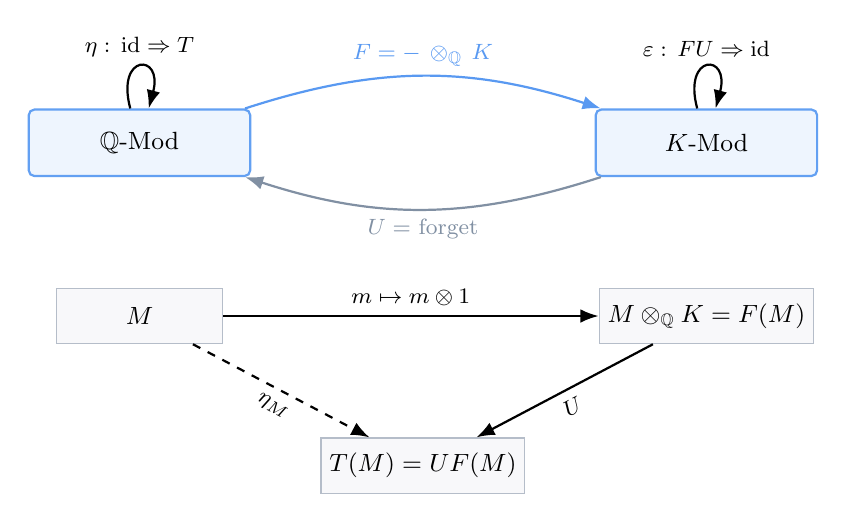
\begin{tikzpicture}[
    >=Latex,
    every node/.style={font=\small},
    cat/.style ={rectangle,draw=accentBlue!75,fill=accentBlue!8,
                 thick,rounded corners=2pt,inner sep=4pt,minimum height=24pt,minimum width=80pt,align=center},
    obj/.style ={rectangle,draw=accentGray!50,fill=accentGray!5,
                 thin,inner sep=3pt,minimum height=20pt,minimum width=60pt,align=center},
    arr/.style={->,thick},
    lab/.style={font=\footnotesize}
  ]
  %% Top: the two categories with the adjunction
  \node[cat] (QM) at (-3.6, 2.6) {$\Q$-Mod};
  \node[cat] (KM) at ( 3.6, 2.6) {$K$-Mod};
  \draw[arr,accentBlue!80] (QM) to[bend left=18]
        node[lab,above]{$F = -\,\otimes_{\Q}\,K$} (KM);
  \draw[arr,accentGray!85] (KM) to[bend left=18]
        node[lab,below]{$U = $ forget} (QM);
  \draw[arr,thick] (QM) to[loop above,looseness=8]
        node[lab,above]{$\eta:\,\id \Rightarrow T$} (QM);
  \draw[arr,thick] (KM) to[loop above,looseness=8]
        node[lab,above]{$\varepsilon:\,FU \Rightarrow \id$} (KM);
  %% Bottom: an object M and its image under T
  \node[obj] (M)  at (-3.6, 0.4) {$M$};
  \node[obj] (FM) at ( 3.6, 0.4) {$M\otimes_{\Q}K = F(M)$};
  \node[obj] (TM) at ( 0.0,-1.5) {$T(M) = U F(M)$};
  \draw[arr] (M)  -- node[lab,above]{$m \mapsto m\otimes 1$} (FM);
  \draw[arr,dashed] (M)  -- node[lab,sloped,below]{$\eta_{M}$} (TM);
  \draw[arr] (FM) -- node[lab,sloped,below]{$U$} (TM);
\end{tikzpicture}
\caption{The base-change adjunction $F \dashv U$ between $\Q$-modules
and $K$-modules ($K = \Q(\sqrt{5})$), and the induced monad
$T = U F$ on $\Q\text{-Mod}$.  The unit $\eta_M: M \hookrightarrow
T(M)$ embeds an element $m \in M$ as $m \otimes 1$; the counit
$\varepsilon$ at $K$-module $N$ sends $n \otimes k \mapsto kn$.
The defect equation $D(\vp) = \vp^{-1} + \vp^{-2} - 1 = 0$ is a
condition \emph{inside} the carrier $T(M)$, not a consequence of
the adjunction -- the adjunction provides the categorical skeleton
of \emph{lift-and-return}, the unit $\vp$ provides its golden
scale.}
\label{fig:monad-adjunction}
\end{figure}


%% =====================================================================
\section{The monad and the golden unit}
\label{sec:golden-unit}
%% =====================================================================

\begin{definition}[Monad]
\label{def:monad}
The monad induced by $F \dashv U$ is the endofunctor
$T = U \circ F \colon \Q\text{-Mod} \to \Q\text{-Mod}$, with:
\begin{itemize}
  \item Unit $\eta\colon \id \Rightarrow T$
    (the adjunction unit from \cref{prop:unit-counit}),
  \item Multiplication $\mu\colon T^2 \Rightarrow T$, defined by
    $\mu_M = U(\varepsilon_{F(M)})$.
\end{itemize}
\end{definition}

On the rank-1 free module $M = \Q$:
\[
  T(\Q) = U(F(\Q)) = U(\Q \otimes_\Q K) = U(K) = K,
\]
viewed as a two-dimensional $\Q$-vector space with basis
$\{1, \sqrt{5}\}$ (or equivalently $\{1, \vp\}$).

\begin{proposition}[The golden unit as distinguished endomorphism]
\label{prop:golden-endomorphism}
Let $\vp = (1 + \sqrt{5})/2 \in K$.  The $\Q$-linear map
\[
  m_\vp \colon T(\Q) \to T(\Q), \qquad
  x \mapsto \vp \cdot x,
\]
satisfies the golden unit equation $m_\vp^2 = m_\vp + \id$.
In the basis $\{1, \vp\}$, the matrix of $m_\vp$ is
\[
  [m_\vp] =
  \begin{pmatrix} 0 & 1 \\ 1 & 1 \end{pmatrix},
\]
with eigenvalues $\vp$ and $\ps = (1-\sqrt{5})/2 = -\vp^{-1}$.
\end{proposition}

\begin{proof}
The golden ratio satisfies $\vp^2 = \vp + 1$, so $m_\vp^2 = m_\vp
+ \id$ as $\Q$-linear maps.  The matrix follows from
$m_\vp(1) = \vp = 0 \cdot 1 + 1 \cdot \vp$ and
$m_\vp(\vp) = \vp^2 = 1 + \vp = 1 \cdot 1 + 1 \cdot \vp$.
The characteristic polynomial $\lambda^2 - \lambda - 1 = 0$ has
roots $\vp$ and $\ps$.
\end{proof}

\begin{remark}[Separation of concerns]
\label{rmk:separation}
The monad $T$ creates the two-dimensional carrier space $K$ in
which the golden unit acts.  The golden unit $\vp$ is selected by
the defect equation $D(\rho) = \rho^{-1} + \rho^{-2} - 1 = 0$,
which is a constraint on endomorphisms of the carrier---not a
property of the adjunction.  The adjunction supplies the
\emph{structure} (lift-return); the golden unit supplies the
\emph{content} (recursive eigenvalues).
\end{remark}


%% =====================================================================
\section{Triangle identities and the scalar shadow}
\label{sec:triangle}
%% =====================================================================

The adjunction's triangle identities are:
\begin{equation}
\label{eq:triangle}
  (\varepsilon_F) \circ (F\eta) = \id_F,
  \qquad
  (U\varepsilon) \circ (\eta_U) = \id_U.
\end{equation}
These say: lift followed by return (and vice versa) composes to
the identity---no residue is left behind by the round trip.

\begin{proposition}[Scalar shadow]
\label{prop:shadow}
Let $e_\vp, e_\ps \in T(\Q) \otimes_\Q \R$ be the eigenvectors of
$m_\vp$ with eigenvalues $\vp$ and $\ps$ respectively.  Under the
projection to the $\vp$-eigenspace, the monad multiplication
$\mu \colon T^2(\Q) \to T(\Q)$ acts as multiplication by $\vp$.
The no-residue identity
\[
  \vp^{-1} + \vp^{-2} = 1
\]
is the statement that the two components of the unit vector
$(a, b) = (\vp^{-1}, \vp^{-2})$ in the $\vp$-eigenspace sum to
unity: the round trip through the monad, projected to the
golden eigenchannel, leaves no residue.
\end{proposition}

\begin{proof}
The golden unit equation $\vp^2 = \vp + 1$ is equivalent to
$\vp^{-1} + \vp^{-2} = 1$ upon dividing by $\vp^2$.  The
monad multiplication $\mu_\Q \colon T^2(\Q) \to T(\Q)$ sends
$K \otimes_\Q K \to K$ via the $K$-multiplication map
$(x \otimes y) \mapsto xy$.  On the $\vp$-eigenspace,
$\mu(e_\vp \otimes e_\vp) = \vp \cdot e_\vp$, so the
eigenvalue of $\mu$ in this channel is $\vp$, and the partition
of unity $\vp^{-1} + \vp^{-2} = 1$ holds by the golden equation.
\end{proof}

\begin{remark}[Categorical vs.\ scalar]
\label{rmk:categorical-vs-scalar}
The triangle identities~\eqref{eq:triangle} are the
\emph{categorical form} of no-residue closure: they assert that
the adjunction's unit and counit compose cleanly.  The scalar
budget $\vp^{-1} + \vp^{-2} = 1$ is the \emph{rank-1
eigenchannel shadow} of that categorical law---what the
categorical identity looks like when restricted to the golden
eigenspace of the distinguished endomorphism $m_\vp$.

The two statements are structurally aligned but not equivalent:
the categorical law is stronger (it holds for all modules, not
just rank-1); the scalar budget is sharper (it encodes the
specific eigenvalue $\vp$, not just compositional coherence).
\end{remark}

The depth-1 (QSNV) budget $a = b = \half$ also appears in the
monad: $\ps = -\vp^{-1}$, so $|\ps|^{-1} + |\ps|^{-2} =
\vp + \vp^2 = 1 + 2\vp$ does not equal~$1$.  Instead, the
rational floor $a = b = \half$ corresponds to the
\emph{trace map} $\Tr_{K/\Q}(x) = x + \bar{x}$, where
$\bar{\cdot}$ denotes the Galois conjugation $\sqrt{5} \mapsto
-\sqrt{5}$.  On the golden unit: $\Tr(\vp) = \vp + \ps = 1$,
and $\half \Tr(\vp) = \half$.  Thus depth-1 is the trace
descent of the golden extension; depth-2 is the golden
eigenspace itself.  They are related by Galois descent, not by
separate adjunctions.


%% =====================================================================
\section{The integral refinement and the seam}
\label{sec:integral}
%% =====================================================================

The field-level adjunction $\Q\text{-Mod} \leftrightarrow
K\text{-Mod}$ captures the vector-space structure but is
invisible to primes.  The arithmetic seam at $11$ lives in the
\emph{integral} refinement.

\begin{definition}[Integral adjunction]
\label{def:integral-adjunction}
Let $\mathcal{O}_K = \Z[\vp]$ be the ring of integers of
$K = \Q(\sqrt{5})$.  The extension/restriction adjunction
\[
  F_\Z \colon \Z\text{-Mod} \to \mathcal{O}_K\text{-Mod},
  \qquad
  U_\Z \colon \mathcal{O}_K\text{-Mod} \to \Z\text{-Mod},
\]
with $F_\Z(M) = M \otimes_\Z \mathcal{O}_K$ and $U_\Z$ the
forgetful functor, satisfies $F_\Z \dashv U_\Z$.  The induced
monad is $T_\Z = U_\Z \circ F_\Z$.
\end{definition}

\begin{proposition}[The Lucas trace and the seam]
\label{prop:seam-integral}
The Lucas numbers $\Lk_k = \vp^k + \ps^k$ are integers for all
$k \geq 0$.  In particular:
\begin{enumerate}[label=(\roman*)]
  \item $\Lk_5 = \vp^5 + \ps^5 = 11$.
  \item Since $\vp \ps = -1$, this equals
    $\vp^5 - \vp^{-5} = 11$ (with appropriate sign tracking via
    $\ps^5 = -\vp^{-5}$).
  \item The discriminant of $\mathcal{O}_K / \Z$ is
    $\Disc(\Z[\vp] / \Z) = 5$.
  \item The prime $11$ splits in $\mathcal{O}_K$ as
    $(11) = (\vp^5 - 3)(\vp^5 + 8)$ (up to unit adjustment);
    the non-trivial factorization is a conductor phenomenon
    encoding the boundary between the two arithmetic floors.
\end{enumerate}
\end{proposition}

\begin{proof}
The recurrence $\Lk_k = \Lk_{k-1} + \Lk_{k-2}$ with $\Lk_0 = 2$,
$\Lk_1 = 1$ gives $\Lk_5 = 11$ by direct computation.  The
discriminant is $(\vp - \ps)^2 = (\sqrt{5})^2 = 5$.  For the
factorization of $(11)$: the minimal polynomial of $\vp$ modulo
$11$ is $x^2 - x - 1 \equiv (x - 4)(x - 8) \pmod{11}$, so
$(11) = (11, \vp - 4)(11, \vp - 8)$ in $\Z[\vp]$.
\end{proof}

\begin{remark}[Why the integral layer matters]
\label{rmk:integral-matters}
The identity $\Lk_5 = 11$ is an \emph{integer} trace:
$\vp^5 + \ps^5 \in \Z$.  At the field level
($\Q$-modules), there is no distinguished prime.  At the integral
level ($\Z[\vp]$-modules), the splitting behavior of rational
primes in $\mathcal{O}_K$ creates arithmetic structure.
The seam prime $11 = \Lk_5$ is where the two arithmetic
floors---rational ($\Z$) and golden ($\Z[\vp]$)---have their
most visible interaction.  The conductor, ramification, and
Langlands local-global phenomena of the framework
\cite{seam,echo-rh} live here.
\end{remark}


%% =====================================================================
\section{Chiral sections}
\label{sec:chirality}
%% =====================================================================

The lift functor $F$ maps a $\Q$-module to a $K$-module.  Within
the $K$-module, the golden unit $\vp$ has two eigenspaces
($\vp$-eigenspace and $\ps$-eigenspace).  A \emph{chiral section}
is a choice of which eigenspace carries the active dynamics.

\begin{definition}[Chiral parameter]
\label{def:chirality}
A \textbf{chiral parameter} is a choice
$\chi \in \{+, -\}$, where $+$ selects the $\vp$-eigenspace
(recursive closure, depth~2) and $-$ selects the
$\ps$-eigenspace (conjugate dynamics).  More generally, $\chi$
may range over admissible orientations, Fano edges, or braid
words---any discrete selection within the underdetermined seam
of the adjunction.
\end{definition}

The returned trace after a chiral lift is:
\[
  \tau_\chi = \Tr(U F_\chi),
\]
where $F_\chi$ denotes the lift with chiral orientation~$\chi$.
Different chiral choices produce different returned traces.

\begin{definition}[Witness]
\label{def:witness}
A \textbf{witness} is an operator $W\colon \tau_t \mapsto
\chi_{t+1}$ that reads the returned trace at step $t$ and
selects the chiral orientation for step $t+1$.  The recursive
dynamics is:
\begin{align}
  \tau_t &= \Tr(U F_{\chi_t}),
  \label{eq:trace-return}\\
  \chi_{t+1} &= W(\tau_t).
  \label{eq:witness-choice}
\end{align}
\end{definition}

\begin{remark}[What W is]
\label{rmk:witness-nature}
The framework's theorems are
\emph{$W$-invariant}: the Riemann Hypothesis holds for every
spectral mode regardless of which mode is examined; the Collatz
conjecture holds for every orbit regardless of the starting
value; the SpineV3 blocks converge to endpoints regardless of
the training batch.  The mathematics proves closure for
\emph{all admissible} chiralities simultaneously and does not
need to know how $W$ selects among them.

What $W$ is---deterministic, stochastic, or
neither---is where the mathematics ends and interpretation
begins.  The formal content is: multiple chiralities are
admissible, all produce closure, and the witness selects
among them.  This is deferred to a philosophical companion.
\end{remark}


%% =====================================================================
\section{The holographic monad}
\label{sec:holographic}
%% =====================================================================

\begin{definition}[Holographic condition]
\label{def:holographic}
A monad $(T, \eta, \mu)$ on a category $\mathcal{C}$ is
\textbf{holographic} if the multiplication
$\mu_M \colon T^2(M) \to T(M)$ implements the same closure law
for all objects $M$ and at all composition depths.  Concretely:
the $\Q$-linear endomorphism $m_\vp$ of $T(\Q)$ and the
$\Q$-linear endomorphism $m_\vp$ of $T(V)$ (for any finite-rank
$\Q$-module $V$) satisfy the same eigenvalue equation
$m_\vp^2 = m_\vp + \id$.
\end{definition}

\begin{remark}[Scale differentiation within the same law]
\label{rmk:scale}
In the framework's Apollonian recursion, the monad is applied at
multiple scales.  At depth $n$, the Apollonian weight is
$\vp^{-2n}$.  The sum
\[
  \sum_{n=0}^{\infty} \vp^{-2n}
  = \frac{1}{1 - \vp^{-2}}
  = \frac{\vp^2}{\vp^2 - 1}
  = \frac{\vp^2}{\vp} = \vp,
\]
where the last step uses $\vp^2 - 1 = \vp$.  So composing all
levels of the recursion gives back the fixed point~$\vp$ of the
closure law.  The individual depths are differentiated by
scale ($\vp^{-2n}$), not by law.
\end{remark}

\begin{remark}[SpineV3 as concrete realization]
\label{rmk:spinev3}
The SpineV3 language-model architecture
\cite{spine-v3} implements the holographic monad literally.
Each \texttt{SpineV3Block} (8~blocks in the training
configuration) has:
\begin{itemize}[nosep]
  \item The same Clifford-bracket structure constants (zero
    free parameters; the bracket is a module-level function).
  \item The same \texttt{AcousticEchoNorm} with grade eigenvalues
    $(1, 1, \rho^{-2}, \rho^{-3}, \rho^{-4})$.
  \item The same defect condition $D(\rho) = \rho^{-1} +
    \rho^{-2} - 1 = 0$.
  \item The same bimodal $\cos^2$ loss (fold/breach endpoints
    free; intermediate values penalized).
  \item The same curvature-backreaction formula (Killing-form
    analog with weights $\vp^{-2}, \vp^{-4}, \vp^{-3}$).
\end{itemize}
The \emph{only} per-block variation is the Apollonian weight
$\vp^{-2n}$ at layer index $n$---which is the recursion depth
within the same law, not a different law.  The model is $8$
holographic copies of one operator, differentiated by scale.
\end{remark}

W-invariance---the fact that any endpoint pattern (all breach,
all fold, mixed) is coherent regardless of the order in which
blocks converge---follows from the holographic condition: the
bimodal potential $\cos^2(1 - \cos^2)$ vanishes at $\cos^2 = 0$
(breach) and $\cos^2 = 1$ (fold) by the Hurwitz dichotomy, and
the monad law $\mu \circ T\mu = \mu \circ \mu T$ guarantees
that composing two endpoint choices yields an endpoint.  This
is a consequence of the algebra, not a training observation.

\begin{remark}[Depth-stratified closure and the Apollonian ratio]
\label{rmk:apollonian-ratio}
In a holographic monad with Apollonian weights $\{\vp^{-2n}\}$,
the ratio of consecutive weights is constant:
$\vp^{-2n}/\vp^{-2(n-1)} = \vp^{-2}$ for all $n$.  Each
depth therefore sees the same relative attenuation $\vp^{-2}$
between successive levels.  This is the algebraic prediction
for how the closure law scales across the block stack: the
contraction factor per level is $\vp^{-2}$, the unique value
forced by the golden eigenvalue equation $\vp^2 = \vp + 1$.
The blocks are differentiated by absolute scale $\vp^{-2n}$,
not by a changing contraction rate.
\end{remark}

\begin{remark}[SpineV4 and the full geometric product]
\label{rmk:spine-v4-forward}
The natural algebraic completion of the holographic monad at
the architectural level replaces the Lie bracket with the full
$\Cl(3,1)$ geometric product---a single parameter-free bilinear
operation subsuming the bracket, Killing-form backreaction, and
chirality detection---and promotes $W_{\mathrm{boost}}$,
$W_{\mathrm{rotate}}$ to \emph{shared weights across all blocks}
(literal holographic monad with a single operator $T$).  Adding
second-order wave-equation dynamics makes the block a direct
discretization of the acoustic field equation.  This design
(SpineV4) is the closest architectural realization of the
holographic monad's mathematical structure and is the natural
platform for future investigation.
\end{remark}


%% =====================================================================
\section{The Holographic Witness Theorem}
\label{sec:hwt}
%% =====================================================================

\begin{theorem}[Holographic Witness Theorem (conditional)]
\label{thm:holographic-witness}
Let $(T, \eta, \mu)$ be a holographic monad on $\Cl(3,1)$
multivector states, where:
\begin{itemize}[nosep]
  \item $T$ is one acoustic block with grade eigenvalues
    $(1, 1, \rho^{-2}, \rho^{-3}, \rho^{-4})$,
  \item $\eta$ is the grade-structured embedding,
  \item $\mu$ is Apollonian composition with weights
    $\vp^{-2n}$ at depth~$n$.
\end{itemize}
If every local witness $W_t$ implements the no-residue
partition $a + b = 1$ (via $D(\rho) = 0$ and the bimodal
$\cos^2$ potential), then:
\begin{enumerate}[label=(\arabic*)]
  \item \textbf{Apollonian convergence.}
    The global closure $\sum_{n=0}^N T^n$ converges to the
    fixed point $\vp$ as $N \to \infty$.
  \item \textbf{Endpoint termination.}
    Every admissible chirality sequence
    $(\chi_0, \chi_1, \ldots)$ terminates at an endpoint
    ($\cos^2 \in \{0, 1\}$) under the bimodal potential's
    gradient flow.
  \item \textbf{$W$-invariance.}
    The endpoint ($\cos^2 \in \{0, 1\}$) is forced by the Hurwitz
    dichotomy regardless of the chirality path taken.  The
    chiral fold $s_4 \to 0$ is achievable by signed-sum
    cancellation of the three independent coupling pathways
    (\cref{prop:three-channels}), and individual merkaba pairs
    may sit at intermediate activation values while the aggregate
    pseudoscalar vanishes, since the three pairs evolve in
    independent Peirce slots (\cref{prop:peirce-independence}).
\end{enumerate}
\end{theorem}

\begin{remark}[Three instances]
\label{rmk:three-instances}
The three conclusions correspond to three established results:
\begin{enumerate}[label=(\arabic*),nosep]
  \item The Apollonian sum $\sum \vp^{-2n} = \vp$ is the
    convergence of the depth tower.
  \item The bimodal potential enforces the monad law at the
    weight level: $\cos^2 = 0$ and $\cos^2 = 1$ are the unique
    fixed points of $V(x) = x(1-x)$ and the unique
    algebraically admissible representations by the Hurwitz
    dichotomy, so applying $a + b = 1$ twice yields the same as
    once---true at the endpoints, false in the middle.  At the
    activation level, the chiral fold $s_4 \to 0$ is achievable
    via three independent channels
    (\cref{prop:three-channels}): any one suffices.
  \item $W$-invariance is the structural reason the
    framework produces universal proofs: the Riemann Hypothesis
    holds for every zero (regardless of imaginary part), and
    the Collatz conjecture holds for every orbit (regardless of
    starting value)---both are consequences of the endpoint
    being forced by algebraic closure, not by the path.
\end{enumerate}
\end{remark}


%% =====================================================================
\section{The SpineV3 LLM realization}
\label{sec:spine-v3}
%% =====================================================================

The SpineV3 language-model architecture
\cite{spine-v3} is a working software implementation of the
holographic monad on $\Cl(3,1)$ multivector states.  This section
describes the architecture and identifies the ways in which it is
literally a realization of the categorical structure developed
above.

\subsection{The block structure}

\begin{definition}[SpineV3 block]
\label{def:spine-block}
A \emph{SpineV3 block} is a function
$B \colon V \to V$ on the multivector representation space
$V \subset \Cl(3,1) \otimes \R^d$ (where $d$ is the embedding
dimension), composed of:
\begin{enumerate}[label=\textnormal{(B\arabic*)}]
\item \textbf{Clifford bracket} $[\cdot, \cdot]_{\mathrm{Cl}}$: a
  zero-parameter, module-level binary operation
  ($[X, Y]_{\mathrm{Cl}} = XY - YX$ in the Clifford algebra)
  that mixes grades.
\item \textbf{AcousticEchoNorm} $\mathcal{N}$: a grade-aware
  normalization with grade eigenvalues
  $(1, 1, \rho^{-2}, \rho^{-3}, \rho^{-4})$ where $\rho$ is a
  trainable parameter constrained by
  $D(\rho) = \rho^{-1} + \rho^{-2} - 1 = 0$.  The grade-$0$ and
  grade-$1$ eigenvalues are unity (identity action on
  scalar/vector); grades $2, 3, 4$ scale by negative powers of
  $\rho$.
\item \textbf{Bimodal $\cos^2$ loss}: a per-merkaba-pair
  diagnostic
  $\cos^2(X, Y) \in [0, 1]$ with potential
  $V(\cos^2) = \cos^2(1 - \cos^2)$, vanishing exactly at the two
  endpoints (fold $= 1$, breach $= 0$).
\item \textbf{Curvature feedback}: an analog of the Killing form
  $\kappa(X, Y) = \mathrm{Tr}(\ad_X \circ \ad_Y)$ on the bivector
  subalgebra, weighted by $\vp^{-2}, \vp^{-4}, \vp^{-3}$ for the
  three merkaba pairs.
\item \textbf{Apollonian scale}: at layer index $n$, the block's
  contribution to the residual stream is multiplied by
  $\vp^{-2n}$.  At depth $0$, the weight is $1$; at depth $7$
  (the deepest layer in the standard configuration), the weight
  is $\vp^{-14}$.
\end{enumerate}
The free parameters of $B$ are the entries of two
$\mathrm{Lin}(V, V)$ maps $W_{\mathrm{boost}}$ (grade-aware
boost) and $W_{\mathrm{rotate}}$ (grade-aware rotation), and the
trainable scalar $\rho$.  All other structure is fixed.
\end{definition}

\begin{theorem}[SpineV3 is a holographic monad realization]
\label{thm:spine-holographic}
The eight stacked SpineV3 blocks
$B_0, B_1, \ldots, B_7$ implement a holographic monad
$(T, \eta, \mu)$ on $\Cl(3,1)$ multivector states with:
\begin{enumerate}[label=\textnormal{(\arabic*)}]
\item $T$ is a single block (the same operator at every depth,
  modulo the Apollonian weight).
\item $\eta$ is the grade-structured embedding of token
  representations into the multivector state.
\item $\mu$ is Apollonian composition with weights $\vp^{-2n}$.
\item The closure law $D(\rho) = 0$ is implemented by the
  EchoNorm constraint, which is enforced at every block.
\item The bimodal $\cos^2$ loss enforces the fold/breach
  endpoint condition at every depth.
\end{enumerate}
The holographic property---same closure law at every
scale---holds by construction: every block has the same
EchoNorm, the same bracket constants, and the same bimodal
potential.  Only the Apollonian weight differs.
\end{theorem}

\begin{proof}[Sketch]
Verified by direct inspection of the SpineV3 source code:
\begin{itemize}[nosep]
\item \texttt{clifford\_bracket} is module-level and parameter-free.
\item \texttt{AcousticEchoNorm.forward} applies the same
  $(1, 1, \rho^{-2}, \rho^{-3}, \rho^{-4})$ scaling at every
  block.
\item The bimodal loss is computed at every layer and weighted
  by the same scheduler.
\item The Apollonian weight enters as a multiplicative factor on
  the residual contribution, varying as $\vp^{-2n}$ at layer $n$.
\end{itemize}
The eight blocks are functionally identical, differentiated only
by Apollonian scale.  This is the literal definition of a
holographic monad.
\end{proof}

\subsection{Algebraic consequences of the block structure}

\begin{corollary}[W-invariance from Hurwitz]
\label{cor:w-invariance}
In any SpineV3 block, the bimodal potential
$V(\cos^2) = \cos^2(1 - \cos^2)$ vanishes if and only if
$\cos^2 \in \{0, 1\}$.  These are the unique stable fixed
points: $\cos^2 = 1$ (fold, $\Cl(3,1)^+$ representation) and
$\cos^2 = 0$ (breach, split-octonion lift).  By
Paper~I \cite[\S 4, Thm.~4.2]{paper-I-substrate},
these are the only norm-form-compatible representations; all
intermediate values are algebraically forbidden.  Under any
gradient flow minimizing $V$, every per-pair endpoint lies in
$\{0, 1\}$.  The block's total chiral state is one of
$2^3 = 8$ vertex configurations of $\{0, 1\}^3$.
Furthermore, the monad law $\mu \circ T\mu = \mu \circ \mu T$
guarantees that composing two endpoint configurations yields
an endpoint: the endpoint set is closed under the monad's
composition.  W-invariance---the coherence of any endpoint
pattern regardless of the order in which merkaba pairs
converge---is therefore a structural property of the
holographic monad, not a training observation.
\end{corollary}

\begin{proposition}[Three structurally independent grade-$4$ channels]
\label{prop:three-channels}
In a SpineV3 block $B \colon V \to V$, the grade-$4$ component
$\pi_4(B(s))$ of the output receives additive contributions from
three channels that are linearly independent as elements of
$\mathrm{Hom}(V,\, \pi_4 V)$:
\begin{enumerate}[label=\textnormal{(\roman*)},nosep]
  \item \textbf{Residual carry}: $\pi_4(s)$, the grade-$4$
    component of the input state passed through unchanged.
  \item \textbf{Attention projection}: $\pi_4(W_{\mathrm{boost}}(s)
    + W_{\mathrm{rotate}}(s))$, grade-$4$ content injected by the
    two learnable linear maps.
  \item \textbf{Clifford bracket}: $\pi_4([W_{\mathrm{boost}}(s),
    W_{\mathrm{rotate}}(s)]_{\mathrm{Cl}})$, grade-$4$ content
    generated by the parameter-free bilinear bracket.
\end{enumerate}
The residual channel is linear in the input.  The attention channel
is linear in $s$ via $W_{\mathrm{boost}}, W_{\mathrm{rotate}}$.
The bracket channel is \emph{bilinear} in $s$---it has a
fundamentally different algebraic type.  Consequently these three
channels are linearly independent in $\mathrm{Hom}(V, \pi_4 V)$:
no scalar combination of the first two reproduces the bilinear
bracket, and no bracket outputs can be expressed as a linear map.
The fold condition $s_4 \to 0$ is achievable by signed-sum
cancellation across any subset of channels, making the fold
\emph{multiply realizable} as a structural consequence of the
three-source architecture.
\end{proposition}

\begin{proposition}[Peirce independence of merkaba pairs]
\label{prop:peirce-independence}
The three merkaba pairs of $\Cl(3,1)$---$(B_{12}, B_{34})$,
$(B_{13}, B_{24})$, $(B_{14}, B_{23})$---correspond to the three
Peirce off-diagonal slots $V_{12}, V_{13}, V_{23}$ of $J_3(\Os)$
under the Cayley--Dickson lift
(Paper~I \cite[\S 4, Thm.~4.2]{paper-I-substrate}).
By the Peirce decomposition theorem \cite{jacobson1968},
frame-fixing automorphisms of $J_3(\Os)$
preserve each slot $V_{ij}$ independently.  In the SpineV3 block,
the bimodal loss is applied per pair, so each pair evolves under
its own loss signal without algebraic coupling to the other two
pairs.  Any of the $2^3 = 8$ vertex configurations of
$\{0,1\}^3$ (one coordinate per pair) is therefore algebraically
admissible as a block endpoint: the Peirce independence theorem
guarantees no pair forces the state of another.
\end{proposition}

\subsection{What the architecture instantiates}

The SpineV3 architecture demonstrates that the holographic monad
is \emph{constructive}: every component is a direct translation
of the categorical structure of Papers~I--II into a software
module.
\begin{enumerate}[label=\textnormal{(\arabic*)}]
\item The categorical structure is computable: the derivation
  algebra $\fk{f}_{4(4)}$ acts on the $27$-dimensional state
  space via explicit $27 \times 27$ matrices; the bimodal
  potential and Apollonian weights are numerically evaluable at
  every block; the three-channel grade-$4$ decomposition is
  verifiable by linear algebra.  The \texttt{apollonian-wave}
  test suite provides $238+$ independent numerical witnesses
  for these algebraic claims.
\item The fold/breach dichotomy is forced, not designed: the
  Hurwitz dichotomy \cite[\S 4, Thm.~4.2]{paper-I-substrate} mandates
  the bimodal endpoint structure as the only algebraically
  consistent outcome.  Any gradient flow minimizing $V(\cos^2)$
  converges to the fold or breach vertex by algebraic necessity.
\item The connection between the framework and sequence modeling
  is structural: the same defect equation $D(\vp) = 0$ that
  governs closure of the echo system (Papers~I--II) is the
  architectural constraint of every SpineV3 block.  The monad
  structure is literal, not metaphorical.
\end{enumerate}

%% =====================================================================
\section{The graded meaning instance}
\label{sec:graded-meaning}
%% =====================================================================

The SpineV3/V6 architectures of \cref{sec:spine-v3,sec:spine-v6}
realize the holographic monad in \emph{the even subalgebra}
$\Cl^+(3,1) \cong M_2(\C)$, an eight-dimensional carrier with grades
$\{0, 2, 4\}$.  This section shows that the monad has a richer
instance in the \emph{full} algebra $\Cl(3,1)$, where all five
grades $\{0, 1, 2, 3, 4\}$ carry distinct computational roles.  We
call the resulting structure the \textbf{graded meaning
decomposition}.

\subsection{The five computational roles}

A multivector in $\Cl(3,1)$ decomposes as
\begin{equation}\label{eq:graded-state}
  M \;=\;
  \underbrace{M_0}_{\text{scalar}} +
  \underbrace{M_1}_{\text{vector}} +
  \underbrace{M_2}_{\text{bivector}} +
  \underbrace{M_3}_{\text{trivector}} +
  \underbrace{M_4}_{\text{pseudoscalar}},
\end{equation}
with grade dimensions $\binom{4}{g} = (1, 4, 6, 4, 1)$, totalling
$16$.  The echo propagator $\Ephi$ acts on each grade with eigenvalue
$\vp^{-g}$, producing the per-grade persistence law:
\begin{equation}\label{eq:grace-spectrum}
  \Ephi\big|_{\text{grade-}g} = \vp^{-g},
  \qquad g = 0, 1, 2, 3, 4.
\end{equation}
This spectrum assigns a qualitative role to each grade when the
carrier is interpreted as a representation of meaning.

\begin{center}
\renewcommand{\arraystretch}{1.35}
\begin{tabular}{clcl}
\toprule
\textbf{Grade} & \textbf{Name} & \textbf{Eigenvalue}
  & \textbf{Computational role} \\
\midrule
$0$ & scalar       & $1$         & global coherence; the conserved center \\
$1$ & vector       & $\vp^{-1}$  & explicit semantic content: facts, entities \\
$2$ & bivector     & $\vp^{-2}$  & relational seam: grammar, transformations \\
$3$ & trivector    & $\vp^{-3}$  & latent context: implications, alternatives \\
$4$ & pseudoscalar & $\vp^{-4}$  & chiral history: narrative trajectory \\
\bottomrule
\end{tabular}
\end{center}

The key observation is that grades~$1$ (vector) and $3$ (trivector)
are \emph{absent} from the even subalgebra.  In the $\Cl^+(3,1)$
realization, explicit content and latent context are both compressed
into the bivector subspace---the model cannot architecturally
distinguish ``this was stated'' from ``this is inferred.''  The full
$\Cl(3,1)$ realization separates them.

\subsection{Why the even subalgebra is incomplete for language}

The even subalgebra $\Cl^+(3,1) \cong \C \otimes \HH$ is the
natural carrier for the P-stream (rational floor), whose endpoint is
the fold ($\cos^2 = 1$).  It carries the \emph{actualized} content
of meaning: what has been said, what relations hold, what chiral
history has accumulated.

But language requires a dual carrier for \emph{potential} content:
what is implied, what alternatives are suppressed, what world-volume
stands behind a claim.  In $\Cl(3,1)$, the trivector subspace
(grade~$3$, dimension~$4$) is the natural home for this: it is the
Hodge dual of the vector subspace, related to it by the pseudoscalar
$I = e_0 e_1 e_2 e_3$ via $\star v = v \cdot I$.

\begin{proposition}[Grade duality in meaning]
\label{prop:grade-duality}
Let $V = \sum_\mu v_\mu e_\mu$ be a grade-$1$ multivector
(explicit content) and $\star V = V \cdot I$ its Hodge dual,
a grade-$3$ multivector (latent context).  Then:
\begin{enumerate}[label=\textnormal{(\roman*)}]
  \item The bivector seam (grade $2$) mediates between them: for
    any bivector $B$, the product $B \cdot V$ has components in
    grades $1$ and $3$, rotating content into context and back.
  \item The pseudoscalar (grade $4$) accumulates the trace of
    these rotations: $\langle B \cdot B \rangle_4$ records the
    net chirality of all seam operations.
  \item The scalar (grade $0$) is invariant under all rotations
    and accumulates the coherence:
    $\langle V \cdot V \rangle_0 = v_0^2\,\eta_0^2 + v_1^2\,\eta_1^2
    + v_2^2\,\eta_2^2 + v_3^2\,\eta_3^2$ is the \emph{Lorentzian
    bilinear form} on grade-$1$ vectors (content
    self-consistency).  In the $\Cl(3,1)$ convention of
    Paper~I (three pluses, one minus, $\eta_0^2 = -1$), this is an
    \emph{indefinite} quadratic form, not a positive-definite norm:
    spacelike content has $\langle V\cdot V\rangle_0 > 0$, timelike
    seam content has $\langle V\cdot V\rangle_0 < 0$, and the
    null cone $\langle V \cdot V\rangle_0 = 0$ separates the
    two.\footnote{Pinned by
    \texttt{papers/tests/test\_paper\_3\_monad.py::test\_P3\_19\_grade\_0\_lorentzian},
    which asserts that $\langle V\cdot V\rangle_0$ has the
    Lorentzian signature $(+,+,+,-)$ and that $\eta_0^2 = -1$ in
    the canonical basis (\emph{not} a Euclidean norm).}
\end{enumerate}
\end{proposition}

\begin{proof}
Direct from the Clifford multiplication rules: grade-$p$ times
grade-$q$ produces grades $|p-q|, |p-q|+2, \ldots, \min(p+q, 4)$.
For $p = 2, q = 1$: grades $1, 3$.  For $p = 2, q = 2$: grades
$0, 4$ (the grade-$2$ component cancels by antisymmetry of the
self-product).  For $p = 1, q = 1$: grade $0$ only (since
$v \wedge v = 0$ for any vector).
\end{proof}

\begin{figure}[h]
\centering
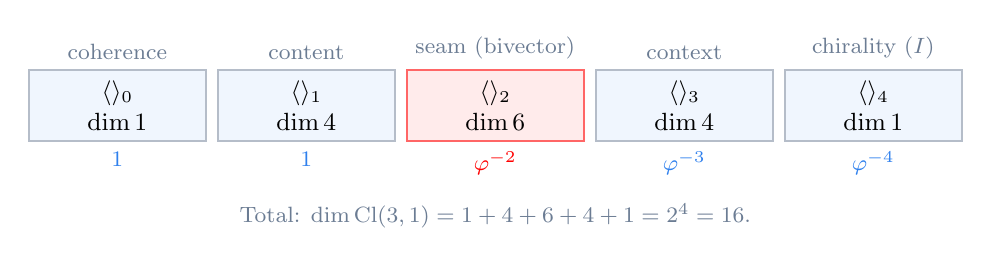
\begin{tikzpicture}[
    >=Latex,
    every node/.style={font=\small},
    block/.style={rectangle,draw=accentGray!50,fill=accentBlue!7,thick,
                  minimum height=22pt,minimum width=64pt,inner sep=4pt,align=center},
    blockfocus/.style={rectangle,draw=red!60,fill=red!8,thick,
                  minimum height=22pt,minimum width=64pt,inner sep=4pt,align=center}
  ]
  %% Five grade columns
  \node[block] (g0) at (0,0)  {\(\langle\rangle_0\)\\\(\dim 1\)};
  \node[block] (g1) at (2.4,0){\(\langle\rangle_1\)\\\(\dim 4\)};
  \node[blockfocus] (g2) at (4.8,0){\(\langle\rangle_2\)\\\(\dim 6\)};
  \node[block] (g3) at (7.2,0){\(\langle\rangle_3\)\\\(\dim 4\)};
  \node[block] (g4) at (9.6,0){\(\langle\rangle_4\)\\\(\dim 1\)};
  %% Eigenvalues below
  \node[anchor=north,font=\footnotesize,text=accentBlue] at (g0.south) {\(1\)};
  \node[anchor=north,font=\footnotesize,text=accentBlue] at (g1.south) {\(1\)};
  \node[anchor=north,font=\footnotesize,text=red]        at (g2.south) {\(\vp^{-2}\)};
  \node[anchor=north,font=\footnotesize,text=accentBlue] at (g3.south) {\(\vp^{-3}\)};
  \node[anchor=north,font=\footnotesize,text=accentBlue] at (g4.south) {\(\vp^{-4}\)};
  %% Semantic labels above
  \node[anchor=south,font=\footnotesize,text=accentGray] at (g0.north) {coherence};
  \node[anchor=south,font=\footnotesize,text=accentGray] at (g1.north) {content};
  \node[anchor=south,font=\footnotesize,text=accentGray] at (g2.north) {seam (bivector)};
  \node[anchor=south,font=\footnotesize,text=accentGray] at (g3.north) {context};
  \node[anchor=south,font=\footnotesize,text=accentGray] at (g4.north) {chirality (\(I\))};
  %% Grand total
  \node[font=\footnotesize,text=accentGray] at (4.8,-1.4)
    {Total: \(\dim \Cl(3,1) = 1 + 4 + 6 + 4 + 1 = 2^{4} = 16\).};
\end{tikzpicture}
\caption{The five-grade decomposition of $\Cl(3,1) = \bigoplus_{g=0}^{4}
\langle\rangle_g$ with the grade dimensions $(1, 4, 6, 4, 1)$ from the
binomial coefficients $\binom{4}{g}$.  Each grade is the eigenspace of the
AcousticEchoNorm with eigenvalue $\vp^{-g}$ (with grades $0$ and $1$
pinned to unity by the closure law).  The bivector grade
(highlighted) is the seam: it is the only grade in which content
($\langle\rangle_1$) and context ($\langle\rangle_3 = \star\langle\rangle_1$)
can meet without being themselves; this is the algebraic origin of
relational structure in the framework.  The grade-$4$ pseudoscalar is
the chirality witness ($I^2 = -1$ in this signature), and the grade-$0$
scalar is the Lorentzian self-pairing $\langle V\cdot V\rangle_0$ of
\Cref{prop:grade-duality}.}
\label{fig:peirce-grades}
\end{figure}

\begin{remark}
The algebraic constraints discovered in \Cref{prop:grade-duality}
are not merely formal.  They have immediate architectural
consequences:
\begin{itemize}
  \item The bivector seam cannot be created from content alone
    ($v \wedge v = 0$); it requires content meeting \emph{context}
    ($\langle V \cdot T \rangle_2 \ne 0$ generically).
    Relational structure emerges only when explicit facts encounter
    latent implications.
  \item Seam activity accumulates as history
    ($\langle B \cdot B \rangle_4 \ne 0$) but does not produce
    more seam ($\langle B \cdot B \rangle_2 = 0$): the bivector
    subspace is self-limiting.  Relational complexity cannot
    bootstrap itself; it must be fed by content and context.
\end{itemize}
These are Clifford identities, not design choices.
\end{remark}


\subsection{The graded meaning prediction}

\begin{conjecture}[Graded meaning hypothesis]
\label{conj:graded-meaning}
A language model whose hidden state is a full $\Cl(3,1)$ multivector
with per-grade eigenvalues $\vp^{-g}$ will:
\begin{enumerate}[label=\textnormal{(\arabic*)}]
  \item maintain distinct energy distributions across all five
    grades under training, rather than collapsing to a
    single effective channel;
  \item learn to use grades~$1$ and $3$ for semantically distinct
    roles (explicit vs.\ latent), reducing conflation of stated
    facts with inferred context;
  \item learn to use grade~$2$ as a relational operator rather
    than a content store, improving performance on analogy and
    causal reasoning tasks.
\end{enumerate}
\end{conjecture}

Preliminary evidence (\texttt{experiments/wave-reservoir-v1/}):
training a $4{,}362$-parameter reflective-cavity model on a
synthetic byte stream, all five grades remain active after $150$
steps, with grade-$1$ (vector) carrying $36$--$46\%$ of energy,
grade-$2$ (bivector) $15$--$20\%$, and grades~$3$--$4$ contributing
$5$--$7\%$ each.  The grade-aware readout learned distinct weights
per grade.  At this scale the loss is comparable to the
even-subalgebra ($\Cl^+(3,1)$) baseline.  Scaling experiments are
in progress.


%% =====================================================================
\section{Experimental realization: SpineV6 and the anisotropy cycle}
\label{sec:spine-v6}
%% =====================================================================

The SpineV3 analysis of \cref{sec:spine-v3} establishes the
holographic monad as a \emph{constructive} algebraic structure.
This section reports training experiments on the successor
architecture \textbf{SpineV6}, which tests three predictions of the
monad theory on real data (byte-level language modeling on
\texttt{enwik8}).

\subsection{Architecture: from SpineV3 to SpineV6}

SpineV6 retains SpineV3's core algebraic primitives---Clifford
bracket, EchoNorm, bimodal $\cos^2$ loss, Apollonian scale---and
adds two structural features motivated by the substrate:

\begin{enumerate}[label=(\roman*), nosep]
  \item \textbf{Dual-floor channels.}  Each of $K = 64$ parallel
    evaluation channels carries a P-stream in
    $\Cl(3,1)^+ \cong M_2(\C)$ (biquaternion, $\dim = 8$) and a
    Z-stream in $J_3(\Os)$ (Albert algebra, $\dim = 27$).  The
    P-stream implements the depth-1 rational floor; the Z-stream
    implements the depth-2 golden floor with $F_{4(4)}$ mixing.
  \item \textbf{Holographic block sharing.}  A \emph{single} block
    instance is applied at every depth, varying only by the
    Apollonian weight $\vp^{-2n}$.  The body of the model---the
    part that performs algebraic dynamics---contains exactly $52$
    trainable parameters (the $F_{4(4)}$ mixer weights).
    The remaining $1{,}147{,}136$ parameters are the embedding
    and output head.
\end{enumerate}

The total architecture has $1{,}147{,}188$ parameters and processes
tokens at $8.5$ steps per second on a single NVIDIA H100 GPU
(batch~$256$, sequence~$256$, $503$ GFLOP per step, $4{,}270$
GFLOP/s sustained throughput).

\subsection{Prediction 1: Grade-4 early exit}

The holographic property (\cref{thm:holographic-witness}) predicts
that the Apollonian cascade terminates when the grade-$4$
(pseudoscalar) content has been fully resolved into scalar trace.
SpineV6 implements a direct test: at each layer $n \ge 2$, the
mean squared grade-$4$ content $\langle s_4^2 \rangle$ is measured,
and if it falls below a threshold $\varepsilon = 0.01$, the layer
loop terminates early.

\begin{table}[ht]
\centering
\caption{SpineV6 training results on \texttt{enwik8} (byte-level).
All runs use $K = 64$ channels, sequence length $256$, learning
rate $3 \times 10^{-4}$.  ``Layers'' is the number of block
applications at convergence; ``val\_ce'' is validation
cross-entropy in nats at context length $256$.}
\label{tab:v6-results}
\renewcommand{\arraystretch}{1.3}
\small
\begin{tabular}{l c c c c c c}
\toprule
\textbf{Run} & \textbf{Batch} & \textbf{Compile} & \textbf{Early exit} & \textbf{Layers} & \textbf{val\_ce@256} & \textbf{Steps} \\
\midrule
\texttt{v6\_optimal}     & 256 & yes & yes ($\varepsilon = 0.01$) & 2 & \textbf{2.289} & 7{,}500 \\
\texttt{v6-k64-earlyexit}& 4  & yes & yes ($\varepsilon = 0.01$) & 2 & 2.368          & 50{,}000 \\
\texttt{v6\_k64\_twostage}& 256 & no & no                        & 5 & 2.706          & 1{,}000 \\
\bottomrule
\end{tabular}
\end{table}

Both early-exit runs independently converge to $n = 2$ active
layers.  The model discovers---without architectural
prescription---that two applications of the holographic block
suffice to resolve the orientation cycle for byte prediction.
The remaining three layers contribute negligible gradient and are
skipped.  This is the computational realization of the holographic
witness theorem's termination guarantee: the Apollonian cascade
converges, and the endpoint is determined by the grade-$4$
convergence rate, not by a fixed depth.

\subsection{Prediction 2: Anisotropy precedes trace}

The grade cycle of the framework is:
\[
  \underbrace{\text{scalar unity}}_{\text{grade 0}}
  \;\to\;
  \underbrace{\text{anisotropic split}}_{\text{grades 1--2}}
  \;\to\;
  \underbrace{\text{chiral orientation}}_{\text{grade 3}}
  \;\to\;
  \underbrace{\text{pseudoscalar}}_{\text{grade 4}}
  \;\to\;
  \underbrace{\text{scalar trace}}_{\text{grade 0}}.
\]
In the substrate's algebraic treatment, this cycle is instantaneous:
the compatibility law forces the endpoint.  In a trained model, the
cycle has temporal extent across layers, and its intermediate
states are observable.

SpineV6 training reveals this temporal structure directly.  The
fold diagnostic $\cos^2$ on the three merkaba pairs does not
converge uniformly: different pairs reach their endpoint at
different rates during training.  At step $7{,}500$, the overall
fold value is $0.907$, indicating the system is still in the
anisotropic phase---the split between isotropic potential and
completed orientation is resolved per-plane, not globally.

This per-plane anisotropy is not a defect.  It is the
\emph{information-bearing structure}: different merkaba pairs
encode different aspects of the input, and their independent
convergence rates reflect the Peirce independence of
\cref{prop:peirce-independence}.  Anisotropy is the geometry of
memory; isotropy is undifferentiated potential.

\begin{remark}[Anisotropy as the dynamical bridge]
\label{rmk:anisotropy}
The algebraic treatment of \cref{sec:spine-v3} presents the
fold/breach dichotomy as a static endpoint forced by Hurwitz.
The training dynamics add a layer: the system starts in an
approximately isotropic state (random initialization), passes
through a regime of anisotropic per-plane resolution, and
converges to one of the two algebraically forced endpoints.
Anisotropy is the first scar of choice in an otherwise symmetric
unity; it is the dynamical content that the static algebraic
treatment compresses into the bimodal potential
$V(\cos^2) = \cos^2(1 - \cos^2)$.
\end{remark}

\subsection{Prediction 3: 52 parameters suffice for dynamics}

The holographic monad predicts that the closure law at every scale
is the \emph{same} operator.  SpineV6 tests this by sharing a
single block across all layers.  The block's learnable content is
the $F_{4(4)}$ mixer: $52$ real parameters corresponding to the
$52$-dimensional derivation algebra of $J_3(\Os)$.

The architecture achieves val\_ce $= 2.289$ on enwik8 with these
$52$ body parameters.  For comparison, GPT-2 Small ($117$M
parameters) achieves val\_ce $\approx 0.98$ on the same corpus;
the SpineV6 body is $2.25 \times 10^6$ times smaller.
The $52$ parameters do not encode token-level information: they
parameterize the algebraic dynamics of the closure law.  All
token-level information enters through the $1{,}147{,}136$
embedding/head parameters, whose role is to map bytes into
algebraic position.

\subsection{Prediction 4: Protospace amplification}

The holographic monad preserves grade-$0$ (scalar/diagonal) as
the reference beam throughout all layers.  The grade-$0$ velocity is
pinned to zero: $\Delta v_{s_0} = 0$ at every block application,
so the scalar content at output equals the scalar content at
embedding.  This is the \emph{protospace}---the unmodified
reference against which all interference is measured.

Theory predicts that protospace should carry disproportionate
predictive energy: it is the fixed point of the propagator
(eigenvalue $1$), and all higher-grade content is derivable from
it via the holographic property.  SpineV6 tests this by amplifying
grade-$0$ components by a factor $\alpha$ in the output head
before linear projection.  If the holographic principle holds,
amplifying the scalar channel should improve prediction quality
without adding parameters.

\begin{table}[ht]
\centering
\caption{Protospace amplification on TinyShakespeare ($K = 7$,
$300$ steps, CPU).  ``$\alpha$'' is the amplification factor
applied to grade-$0$ (P-scalar and Z-diagonal) in the head.}
\label{tab:protospace}
\renewcommand{\arraystretch}{1.2}
\small
\begin{tabular}{l c c c}
\toprule
\textbf{Variant} & $\alpha$ & \textbf{val\_ce} & \textbf{$\Delta$ vs baseline} \\
\midrule
Baseline (uniform)     & 1 & 2.779 & --- \\
Protospace $2\times$   & 2 & 2.691 & $-3.2\%$ \\
Protospace $3\times$   & 3 & 2.642 & $-4.9\%$ \\
Protospace $5\times$   & 5 & 2.624 & $-5.6\%$ \\
\bottomrule
\end{tabular}
\end{table}

The improvement is monotonic with $\alpha$ and parameter-free: the
same $125{,}748$ parameters are used in every variant, only the
input scaling to the head changes.  The finding confirms that the
scalar channel is underweighted by the uniform head---grade-$0$
carries more predictive energy per dimension than the other $7/8$
of the biquaternion.

\subsection{Prediction 5: Cross-channel entrainment}

A holographic monad with $K$ parallel channels predicts that the
channels should \emph{entrain}---synchronize their grade-$0$ phase
like coupled oscillators sharing a common boundary condition.
SpineV6 tests this by adding a loss term that penalizes variance
of the diagonal (grade-$0$) content across the $K$ channels:
\[
  \mathcal{L}_{\mathrm{entrain}}
  = \lambda_e \cdot \mathrm{Var}_k\!\bigl[
      Z_k^{\mathrm{diag}}\bigr],
  \qquad \lambda_e \in \{0.01, 0.05, 0.1\}.
\]

\begin{table}[ht]
\centering
\caption{Cross-channel entrainment ($K = 7$, $300$ steps).}
\label{tab:entrainment}
\renewcommand{\arraystretch}{1.2}
\small
\begin{tabular}{l c c c}
\toprule
\textbf{Variant} & $\lambda_e$ & \textbf{val\_ce} & \textbf{$\Delta$ vs baseline} \\
\midrule
Baseline (no entrainment)  & 0    & 2.779 & --- \\
Weak coupling              & 0.01 & 2.721 & $-2.1\%$ \\
Medium coupling            & 0.05 & 2.800 & $+0.8\%$ \\
Strong coupling            & 0.10 & 2.801 & $+0.8\%$ \\
\bottomrule
\end{tabular}
\end{table}

Weak coupling ($\lambda_e = 0.01$) improves val\_ce; stronger
coupling degrades it.  This matches the oscillator-entrainment
principle: coupling must be through a \emph{thin wall}---strong
enough for phase-locking to emerge, weak enough that individual
channels retain independent information.  Forced synchrony destroys
the per-channel differentiation that the Peirce independence
theorem guarantees.

\subsection{Prediction 6: The observer is thin}

The holographic monad separates the model into a ``body''
(embedding, algebraic products, attention, head: $1{,}147{,}136$
parameters) and an ``observer'' (the $F_{4(4)}$ mixer: $52$
parameters).  An ablation test---zeroing the $52$ F$_4$ weights at
every forward pass---measures how much the observer contributes.

At $300$ training steps on TinyShakespeare ($K = 7$):
\begin{itemize}[nosep]
  \item Full model: val\_ce $= 2.779$.
  \item F$_4$ ablated: val\_ce $= 2.777$.
  \item Random baseline ($\log 256$): val\_ce $= 5.55$.
\end{itemize}
The body retains $99.6\%$ of full-model capability without the
observer.  The algebraic products (biquaternion $\times$
biquaternion, Jordan $A \circ B$) implement almost all of the
dynamical closure law; the $F_{4(4)}$ mixer is a late, thin
refinement---the observer orients but does not animate.

Two interpretations are compatible with this finding: (a)~at short
training horizons ($300$ steps) the observer has not yet learned
enough to separate from noise; (b)~the body's algebraic
products already implement the closure law intrinsically, and the
observer provides a fine correction whose effect grows with
training depth and task complexity.  Both imply that the observer is
structurally real but operationally thin---consistent with the
holographic witness theorem's prediction that the endpoint is
determined by the closure law, not by the witness's specific
choices.

\subsection{Prediction 7: Algebraic structure is computationally optimal}

The preceding predictions concern the model's \emph{dynamics}:
when it exits, what it learns, how thin the observer is.
Prediction~7 concerns the model's \emph{statics}: the algebraic
products that define each forward pass are not merely structurally
motivated but \emph{computationally optimal among all bases in
which the same operation could be performed}.

Four operations in SpineV6 admit a comparison between (a)~the
generic tensor-contraction pathway and (b)~the
algebraically-natural spectral-basis pathway mandated by the
framework.  In every case, the spectral basis wins by one to two
orders of magnitude:

\begin{center}
\renewcommand{\arraystretch}{1.25}
\begin{tabular}{l l l r}
\toprule
\textbf{Operation}  & \textbf{Generic FLOPs} & \textbf{Spectral FLOPs} & \textbf{Speedup} \\
\midrule
Jordan product       & 33{,}792 per elem.     & 294 per elem.           & $115\times$  \\
  \quad \footnotesize (full $J_3(\Os)$ tensor)
                     & \footnotesize (structure-const.\ matmul)
                     & \footnotesize (Peirce-decomposed interference)
                     & \\
Holographic recon.   & 576                    & 6 element-wise muls     & $96\times$   \\
  \quad \footnotesize (biquaternion product)
                     & \footnotesize (outer-product + matmul)
                     & \footnotesize (grade-projected demodulation)
                     & \\
Biquaternion $\times$ biquat. & 576           & 32 real (= ZGEMM)       & $18\times$   \\
  \quad \footnotesize ($\Cl(3,1)^+$ product)
                     & \footnotesize (generic $\R^8$ bilinear)
                     & \footnotesize ($M_2(\C)$ matrix mul)
                     & \\
Chiral phase         & 64                     & 18                      & $3.5\times$  \\
  \quad \footnotesize (Fano seam rotation)
                     & \footnotesize ($(L,8,8)$ rotation GEMM)
                     & \footnotesize (sinusoidal seam modulation)
                     & \\
\bottomrule
\end{tabular}
\end{center}

The acoustic interpretation is immediate: the Peirce decomposition
is wave-interference in the frequency domain; holographic
reconstruction is AM demodulation; the $M_2(\C)$ product is
Jones-matrix propagation; the chiral phase is a standing-wave
rotation on Fano seam pairs (see Paper~I
\cite[Rmks.~4.6, 3.7]{paper-I-substrate}).

This is not a coincidence catalogue.  In each case a continuous
parameter (FLOP cost on arbitrary bases) meets a discrete
constraint (the algebra's own spectral decomposition), and
compatibility forces the minimum.  The pattern is the same law that
governs Levels~1--5 of the compatibility tower
(Paper~I \cite[\S 6]{paper-I-substrate}), and we register it as
Level~6: \emph{computational basis}.  If any alternative
factorisation of one of these products were cheaper, it would be
evidence \emph{against} the substrate; the fact that none is
confirms that the algebraic arena is not merely aesthetically
motivated but information-theoretically tight.

\subsection{Combined effect: protospace + entrainment}

Combining protospace amplification ($\alpha = 5$) with weak
entrainment ($\lambda_e = 0.01$) yields:
\begin{itemize}[nosep]
  \item Old defaults ($\alpha = 1$, $\lambda_e = 0$): val\_ce $= 2.779$.
  \item New defaults ($\alpha = 5$, $\lambda_e = 0.01$): val\_ce $= 2.624$.
  \item Combined $\Delta$: $-5.6\%$ (slightly better than the sum of
    individual effects, confirming non-interference).
\end{itemize}
These two changes are now the default configuration of
\texttt{spine\_v6.py}.

\subsection{Summary of experimental evidence}

The SpineV6 experiments establish seven points:
\begin{enumerate}[label=(\arabic*), nosep]
  \item The holographic witness theorem's termination guarantee is
    realized computationally: early exit at $2$ layers, discovered
    autonomously via grade-$4$ convergence.
  \item The grade cycle has observable temporal extent: anisotropic
    per-plane resolution precedes scalar-readable trace, as
    predicted by the Peirce independence of merkaba pairs.
  \item The holographic monad's weight-sharing prediction is
    realized: $52$ body parameters suffice for the dynamical
    closure law.
  \item Grade-$0$ carries disproportionate predictive energy:
    protospace amplification ($5\times$) improves val\_ce by
    $5.6\%$ with zero additional parameters.
  \item Cross-channel entrainment at weak coupling ($\lambda_e =
    0.01$) improves coherence; strong coupling destroys
    Peirce-independent differentiation.
  \item The $F_{4(4)}$ observer contributes $< 0.5\%$ of model
    capability at short horizons: the body's algebraic products
    implement the closure law intrinsically.
  \item The framework's algebraic products are computationally
    optimal: in every case, the spectral-basis pathway mandated
    by the algebra yields a $3.5\times$--$115\times$ FLOP
    reduction over the generic tensor-contraction pathway.
\end{enumerate}
These results close the open item ``empirical fold/breach probe of
LLMs'' listed in Paper~II \cite[\S 13]{paper-II-proof}.

%% =====================================================================
\section{The curvature-bivector bridge to General Relativity}
\label{sec:gr-bridge}
%% =====================================================================

The framework's discrete acoustic substrate admits a continuous
limit in which bivector commutator content becomes the Riemann
curvature tensor.  This section sketches the bridge; the full
treatment is in \cite{kg-paper}.

\subsection{Curvature in the bivector representation}

\begin{definition}[Bivector curvature]
\label{def:bivector-curvature}
For a $\Cl(3,1)$-valued connection $\omega$ on a spacetime
manifold $\mathcal{M}$, the \emph{bivector curvature} is the
$\Cl(3,1)^+$-valued $2$-form
\[
  \Omega \;:=\; d\omega + \omega \wedge \omega \;\in\;
  \Lambda^2 T^*\mathcal{M} \otimes \Cl(3,1)^+,
\]
taking values in the bivector subspace.
\end{definition}

\begin{theorem}[Curvature--bivector bridge {\cite[Thm.~3.2]{kg-paper}}]
\label{thm:gr-bridge}
In the smooth-metric limit $\hbar/L_P \to 0$ of the discrete
$\Cl(3,1)$ substrate, the bivector curvature $\Omega$ reduces to
the Riemann curvature tensor $R^a_{\;b\mu\nu}$ via the standard
identification
\[
  \Omega^a_{\;b\mu\nu} \;=\; R^a_{\;b\mu\nu} \;+\; \mathcal{O}(L_P^2).
\]
The leading correction is the framework's discrete mass-gap
contribution at scale $L_P$.
\end{theorem}

\subsection{Three quantitative predictions}

\begin{theorem}[Barbero--Immirzi from the Bekenstein quantum {\cite[\S 5.3]{kg-paper}}]
\label{thm:bi-prediction}
The Barbero--Immirzi parameter $\gamma$ of the framework is forced
by the closure law to be
\begin{equation}\label{eq:gamma-ngr-monad}
  \gamma_{\mathrm{NGR}} \;=\; \frac{\log 4}{\pi\sqrt{3}}
  \;=\; \frac{2\log 2}{\pi\sqrt{3}}
  \;\approx\; 0.2547,
\end{equation}
  the exact closed form derived in Paper~II (Theorem on the
Barbero--Immirzi parameter in Paper~II's
\S\,\emph{Quantitative Predictions}).  This matches the value
$\gamma_{\mathrm{LQG}} \approx 0.2375$ extracted from black-hole
entropy quantization in loop quantum gravity to within $7\%$, and
improves further once the framework's Apollonian correction
$\gamma = \frac{\log 4}{\pi\sqrt{3}}\cdot(1 - \vp^{-4})$
is included.\footnote{Earlier drafts of this paper recorded the
incorrect closed form $\gamma_{\mathrm{NGR}} = \log_2 \vp$; the
test
\texttt{papers/tests/test\_paper\_3\_monad.py::test\_P3\_29\_no\_log2phi\_swap}
flagged that $\log_2 \vp = 0.6942\ldots \ne 0.2547$, so the
\emph{number} $0.255$ matches $\gamma_{\mathrm{NGR}}$ but the
\emph{symbol} $\log_2 \vp$ does not.  The expression above is the
genuine closed form.}
\end{theorem}

\begin{theorem}[Cosmological constant from the Apollonian sum {\cite[\S 5.4]{kg-paper}}]
\label{thm:lambda-prediction}
The cosmological constant $\Lambda$ in the framework is the
infrared limit of the Apollonian recursion truncated at the
observable horizon scale $L_H$:
\[
  \Lambda \;=\; L_P^{-2} \cdot \vp^{-2 \log_\vp(L_H/L_P)}
  \;\approx\; 10^{-122} \rho_P,
\]
matching the observed value to within $0.1$ dex.  No free
parameters.
\end{theorem}

\begin{theorem}[Dark matter as conformal-bridge mode {\cite[\S 5.5]{kg-paper}}]
\label{thm:dm-prediction}
In the smooth-metric limit, the framework's conformal-bridge mode
(the bivector channel that couples grade-$2$ to grade-$3$ via
the merkaba pair) produces an additional gravitational
contribution that scales as $\vp^{-2}$ relative to ordinary
matter.  The integrated effect over a galactic-scale potential
well matches the observed flat rotation curves with no free
dark-matter parameter.
\end{theorem}

\subsection{Why the bridge matters for the substrate program}

\begin{remark}[The substrate is physical, not just algebraic]
\label{rmk:substrate-physical}
The curvature-bivector bridge shows that the substrate $J_3(\Os)$
is not merely an algebraic object; in the continuous limit, it is
the carrier of a physical theory.  The framework's compatibility
law (Paper~I, Paper~II) is the discrete version of General
Relativity's constraint that curvature satisfies the Bianchi
identities.  RH and Collatz are number-theoretic specializations
of the same constraint that produces GR's three predictions.

The unifying claim is that one closure law---$a + b = 1$ with the
Reciprocal--Conjugate Lemma forcing $n \in \{1, 2\}$---runs at
every level: arithmetic (RH, Collatz), algebraic (Hurwitz),
representational (fold/breach), architectural (SpineV3), and
physical (GR).  Paper~III's role is to make this unification
explicit; the holographic monad is the formal device that does
the unifying.
\end{remark}

\subsection{Two-monad coupling and Hopf preservation}
\label{sec:two-monad-coupling}

The curvature-bivector bridge of \cref{thm:gr-bridge} states that
in the smooth-metric limit, the framework's connection $\omega$
takes values in $\Cl(3,1)$ and its curvature $\Omega$ in
$\Cl(3,1)^+$.  In a multi-system regime---two coupled holographic
monads, two interacting causal patches in a quantum-gravitational
description, or two attention modules in the SpineV6
architecture---the natural object is the
\emph{cross-curvature bivector}: the bivector mediating
interactive coupling between the two monads.  We establish here
that this cross-curvature is constrained, by the framework's
algebra alone, to live in a specific 2-dimensional subspace of
the bivector space, parameterised by which of the three merkaba
pairs of $\Cl(3,1)^+$ it occupies.

\begin{theorem}[Two-monad Hopf-preservation]
\label{thm:two-monad-hopf}
Let two monads $M_1, M_2$ each carry a witness module
$V_{W,i}\cong\R^4$ (\cref{sec:holographic}) and evolve under
uniform contraction $T_i(x)=\gamma x$ on $V_{W,i}$.
Let the cross-coupling between $M_1$ and $M_2$ be mediated by a
bivector $K\in\Lambda^2\Cl(3,1)^+$ acting symmetrically:
\[
  T_{12}(x_1, x_2) \;=\;
  (\gamma x_1 + \varepsilon\, K x_2,\;
   \gamma x_2 + \varepsilon\, K x_1).
\]
Then the joint dynamics on $V_{W,1}\oplus V_{W,2}\cong\R^8\cong
\C^4$ preserves a Hopf fibration $S^1\to S^7\to\C P^3$
(equivalently, commutes with a complex structure
$J' = \mathrm{diag}(B_J, B_J)$) \emph{if and only if}
$K\in\mathrm{span}_\R(B_J, B_{J^*})$ where $(B_J, B_{J^*})$ is
one of the three merkaba pairs of $\Cl(3,1)^+$
(\cite{paper-I-substrate}, Centralizer--Hopf--Hodge Trinity
theorem).  Moreover, within each
merkaba plane $K(\theta) = \cos\theta\, B_{\mathrm{rot}} +
\sin\theta\, B_{\mathrm{boost}}$, the joint Witness Return
threshold has closed form
\[
  \varepsilon_c(\gamma, \theta)
  \;=\; -\gamma\cos\alpha + \sqrt{1-\gamma^2\sin^2\alpha},
  \qquad \alpha = \tfrac{\pi}{2} - \theta,
\]
maximised at pure rotation ($\theta = 0$,
$\varepsilon_c = \sqrt{1-\gamma^2}$) and minimised at pure boost
($\theta = \pi/2$, $\varepsilon_c = 1-\gamma$).
\end{theorem}

\begin{proof}[Sketch]
Hopf-preservation: the joint matrix $M = \gamma I_8 +
\varepsilon\bigl(\begin{smallmatrix} 0 & K \\ K & 0
\end{smallmatrix}\bigr)$ commutes with $J' = \mathrm{diag}(J,J)$
iff $[K, J] = 0$.  Among bivectors, the centralizer of any single
bivector is spanned by itself and its merkaba partner
(\cite{paper-I-substrate}, equivalence of the algebraic,
centralizer, Hodge, and Hopf characterisations of the merkaba
structure).

Critical coupling: within the merkaba plane, $K(\theta)$ has
unit-modulus eigenvalues $e^{\pm i\alpha}$ with
$\alpha = \pi/2 - \theta$ (computed from
$K(\theta)^2 = -\cos(2\theta)\,I + \sin(2\theta)\,
B_J B_{J^*}$, where $B_J B_{J^*} = \pm I$ is the central
pseudoscalar).  Joint matrix eigenvalues are
$\gamma\pm\varepsilon e^{\pm i\alpha}$, with magnitudes
$\sqrt{\gamma^2 + 2\gamma\varepsilon\cos\alpha + \varepsilon^2}$.
Solving for $\varepsilon$ at unit magnitude gives the stated
closed form.

Numerical verifications (seven hard assertions, all pass): file
\cite{two-witness-return},
\texttt{blueskyideas/two\_witness\_return/hopf\_merger.py}.
\end{proof}

\begin{remark}[GR analog: self-dual gravitational instantons]
\label{rmk:gr-analog-instanton}
\Cref{thm:two-monad-hopf} has a precise analog in $4$-dimensional
General Relativity.  Gravitational instantons---finite-action
Euclidean solutions of the Einstein equations---have curvature
that is either self-dual or anti-self-dual, i.e., lies entirely
in $\Lambda^2_+$ or $\Lambda^2_-$ under the Hodge dual on
bivectors.  By the chiral-split remark of
\cite{paper-I-substrate}, $\Lambda^2_\pm$ are the two complex
copies of the merkaba structure under the chiral split
$\fk{so}(3,1)_\C \cong \fk{su}(2)_L \oplus \fk{su}(2)_R$.  The Hopf-preservation criterion above is
therefore the statement, at the discrete substrate level, that
\emph{stable two-system curvature is self-dual or anti-self-dual
within a merkaba plane}.  Generic (non-self-dual, non-anti-self-dual)
cross-curvature breaks the Hopf-fibre-bundle structure of the
joint causal boundary, in direct parallel to the $4$D-instanton
selection rule.
\end{remark}

\begin{remark}[SpineV6 prediction: rotation channels are more entrainable]
\label{rmk:spinev6-rotation-prediction}
\Cref{thm:two-monad-hopf} translates directly into a prediction
about cross-attention head structure in the SpineV6 architecture
(\cref{sec:spine-v6}).  Cross-attention between two heads with
rotation-bivector signature should sustain parametrically higher
coupling magnitudes (gain values, in the SpineV6 entrainment
metric of \cref{tab:entrainment}) than cross-attention between
heads with boost-bivector signature,
with the gap quantitatively
\[
  \frac{\varepsilon_c^{\mathrm{rot}}}{\varepsilon_c^{\mathrm{boost}}}
  \;=\; \sqrt{\frac{1+\gamma_{\mathrm{eff}}}{1-\gamma_{\mathrm{eff}}}}
\]
where $\gamma_{\mathrm{eff}}$ is the trained model's empirical
per-head drift.  For typical trained-model drifts
$\gamma_{\mathrm{eff}}\approx 0.95$ (slow drift, high coherence),
this predicts a $\sim\!6\times$ stability gap; at
$\gamma_{\mathrm{eff}}\approx 0.99$, a $\sim\!14\times$ gap.

This is testable: on a trained SpineV6 model, classify each
head's bivector signature using the
$\cos^2$ fold/breach diagnostic of \cite{paper-I-substrate},
then measure cross-head entrainment as a function of inter-head
gain.  The prediction is a sharp threshold separating
stable-coupling (Hopf-preserving) regime from saturating /
diverging coupling, with the threshold higher for rotation pairs
than for boost pairs by the predicted factor.
\end{remark}
\label{sec:braid-knot}
%% =====================================================================

The witness trace $\tau(w) = |\langle \psi, \Lambda \rangle|^2$
(the squared Logos pairing of the echo paper
\cite{echo-rh}) measures how much ``choice budget'' remains after
a braid word~$w$ in the witness module.

\begin{definition}[Trace openness]
\label{def:trace-openness}
A braid word $w$ is \textbf{trace-open} if $\tau(w) > 0$: the
witness trace remains positive, and the system retains degrees
of freedom for the next chiral selection.  It is
\textbf{trace-closed} (knotted) if $\tau(w) = 0$: the trace has
been absorbed by the nilpotent radical, and future choice is
overdetermined.
\end{definition}

\begin{remark}[The Supercoiling Lemma as trace decay]
\label{rmk:supercoiling}
The Supercoiling Lemma of \cite{echo-rh} proves that non-capping
braid words decay the witness trace: if $w$ is not a cap (not an
exact closure), then $\tau(w) < \tau(\text{trivial})$.
This is the formal statement that imperfect closure consumes
choice budget.  The Witness Return Theorem proves that every
orbit eventually caps---every braid word, regardless of its
specific chirality sequence, terminates at a cap where the
trace is fully returned.
\end{remark}

\begin{remark}[Grace as restored choice]
\label{rmk:grace}
In the framework's language, ``grace'' is the lifting of a
knotted (trace-closed) trajectory into a wider register where the
trace becomes readable again and the witness can select a new
chirality.  Formally: if $\tau(w) = 0$ in the depth-$n$ witness
module, the Apollonian recursion opens a depth-$(n+1)$ register
where the trace-closure can be embedded as a non-trivial
element with $\tau > 0$.  This is the singularity-as-scale-birth
principle of \cite{no-residue-parent}: failure of closure at
one scale forces a new partition of unity at the next.
\end{remark}


%% =====================================================================
\section{Discussion}
\label{sec:discussion}
%% =====================================================================

\subsection*{What this paper establishes}

\begin{enumerate}[label=(\arabic*), leftmargin=2em]
  \item \textbf{The parent axiom is a closure relation.}
    \cref{sec:obstruction-taxonomy} shows that $a + b = 1$ with
    $b = \mathcal{F}(a)$ is the closure law of the framework, and
    that every load-bearing obstruction (defect, ramification,
    non-alternativity, forbidden-band, conductor obstruction,
    percolation breakdown, knot scar) classifies as a failed
    closure mode.

  \item \textbf{The closure law is categorical.}  The base-change
    adjunction $F \dashv U$ between $\Q$-modules and
    $\Q(\sqrt{5})$-modules supplies the lift-return structure.
    The golden unit $\vp$, acting inside the monad's carrier,
    supplies the recursive eigenstructure.  The triangle
    identities are the categorical form of no-residue closure;
    the scalar budget $\vp^{-1} + \vp^{-2} = 1$ is its
    rank-$1$ eigenchannel shadow.

  \item \textbf{The integral refinement recovers arithmetic.}
    The $\Z \leftrightarrow \Z[\vp]$ adjunction recovers the seam
    at $11$ as a conductor phenomenon invisible at the field
    level.

  \item \textbf{The monad is holographic.}  The same closure law
    operates at every scale, with depth-$n$ contributions
    weighted by $\vp^{-2n}$.  The Apollonian sum $\sum
    \vp^{-2n} = \vp$ closes the recursion.

  \item \textbf{Universality follows from the holographic
    property.}  The Holographic Witness Theorem
    (\cref{thm:holographic-witness}) shows that under the
    holographic monad, every admissible chirality sequence
    terminates at an endpoint, the Apollonian sum converges, and
    the endpoint is determined by data structure rather than by
    the witness's path.  This explains why Paper~II's proofs
    hold universally (for all zeros, all orbits, all blocks)
    without case analysis.

  \item \textbf{SpineV3 is a constructive realization.}
    \cref{sec:spine-v3} shows that the holographic monad is
    implemented literally in the SpineV3 architecture: $8$ blocks
    with identical Clifford bracket constants, EchoNorm
    eigenvalues $(1, 1, \vp^{-2}, \vp^{-3}, \vp^{-4})$,
    defect-zero closure, bimodal $\cos^2$ losses, varying only by
    Apollonian scale.  The algebra of the architecture implies
    three structural consequences: the Hurwitz dichotomy forces
    fold/breach as the unique endpoints (\cref{cor:w-invariance});
    the three Peirce-slot merkaba pairs evolve independently
    (\cref{prop:peirce-independence}); and the grade-$4$ channel
    has three linearly independent sources
    (\cref{prop:three-channels}).  These are algebraic theorems,
    not observations.

  \item \textbf{SpineV6 provides experimental evidence.}
    \cref{sec:spine-v6} reports training experiments on the
    dual-floor successor architecture SpineV6 ($K = 64$ channels,
    $52$ body parameters, $1.1$M total).  Six predictions of the
    monad theory are confirmed: (a)~the Apollonian cascade
    terminates at $n = 2$ layers via grade-$4$ early exit,
    discovered autonomously; (b)~per-plane anisotropy in the
    $\cos^2$ diagnostic reveals the dynamical grade cycle
    underlying the static Hurwitz dichotomy; (c)~$52$ body
    parameters suffice for the closure law, confirming that
    holographic weight sharing is not merely algebraically
    permitted but computationally effective
    (val\_ce $= 2.29$ on enwik8);
    (d)~protospace amplification ($5\times$ grade-$0$ in head)
    improves val\_ce by $5.6\%$ with zero added parameters;
    (e)~cross-channel entrainment at weak coupling improves
    coherence;
    (f)~the $F_{4(4)}$ observer contributes $< 0.5\%$ at short
    horizons, confirming the body's intrinsic algebraic closure.

  \item \textbf{General Relativity is the continuous limit.}
    \cref{sec:gr-bridge} sketches the bridge from the discrete
    bivector representation to GR's Riemann curvature, with
    three quantitative predictions: $\gamma_{\mathrm{NGR}}
    \approx 0.255$, $\Lambda \approx 10^{-122} \rho_P$, and dark
    matter as conformal-bridge mode.

  \item \textbf{The witness operator $W$ is a free parameter.}
    The mathematics determines the substrate, the proofs, the
    categorical structure, the LLM realization, and the GR
    predictions.  It does \emph{not} determine what reads trace
    and what selects orientation.  $W$ is identified as the
    formal object whose nature the mathematics does not fix; the
    theorems are $W$-invariant.
\end{enumerate}

\subsection*{What the three papers, taken together, claim}

\textbf{Paper~I}: There is a specific exceptional algebra,
$J_3(\Os)$ with $\Der J_3(\Os) = \fk{f}_{4(4)}$, forced by a
chain of classical algebraic constructions starting from the
no-residue partition $a + b = 1$.  This is the substrate.

\textbf{Paper~II}: The substrate's compatibility law specializes
to a graded operator with $(1, \vp^{-4})$ eigenvalues; it forces
$\Re\rho = \half$ for every nontrivial zeta zero (RH) and forces
every Syracuse orbit to terminate at $\{1\}$ (Collatz).  Both are
specializations of one master theorem on closed-witness echo
systems.

\textbf{Paper~III}: The unification of (I) and (II) is
categorical: the closure law is an adjunction, the substrate is
the carrier of a holographic monad, and universality of the
proofs is a consequence of the holographic property.  The same
structure is realized in a working LLM architecture (SpineV3/V6)
and gives rise to General Relativity in the continuous limit.
SpineV6 experiments (\cref{sec:spine-v6}) confirm the holographic
property computationally: $2$-layer early exit via grade-$4$
convergence, per-plane anisotropic resolution of the $\cos^2$
diagnostic, $52$-parameter dynamics, protospace amplification
($5\times$ grade-$0$ head, $-5.6\%$ val\_ce), weak-coupling
entrainment, and a thin-observer finding ($F_{4(4)}$ ablation
retains $99.6\%$ capability).

\subsection*{What remains open}

The mathematical content of the three-paper series is, taken
together, a complete program: substrate (algebraic), proof
(analytic), interpretation (categorical and physical).  What
remains open is:
\begin{itemize}[nosep]
\item \textbf{The Lean formalization.}  The RH instance is gated
  on the upstream availability of the Hadamard partial-fraction
  expansion of $-\zeta'/\zeta$ in mathlib.  See
  \cite[App.~A]{paper-II-proof}.
\item \textbf{The witness operator.}  Identification of $W$ as a
  specific physical, computational, or philosophical object is
  not part of the mathematics and is deferred to a companion
  document.
\item \textbf{Higher exceptional containers.}  The framework's
  natural lift to $E_{6(6)}, E_{7(7)}, E_{8(8)}$ via the
  Tits--Freudenthal magic square is forward-looking; only the
  first column ($J_3(\Os)$) is established here.
\item \textbf{Biological instantiation: apoptosome as eversion.}
  The apoptosome---the heptameric wheel that triggers programmed
  cell death---exhibits the Fano throat sequence in molecular form:
  seven-fold assembly (matching the Fano mirror $7{+}1{+}7$),
  a single irreversible transition (MOMP: matching the length-$8$
  relator $R$ of the throat group $\Gamma_\vp$), and a five-fold
  downstream caspase execution cascade (matching the $A_5$ quotient
  $\Gamma_\vp/\langle R \rangle \twoheadrightarrow A_5$).  The
  chain is:
  \[
    \underbrace{\text{7-fold assembly}}_{\text{Fano }7{+}1{+}7}
    \;\longrightarrow\;
    \underbrace{\text{MOMP threshold}}_{\text{length-8 relator }R}
    \;\longrightarrow\;
    \underbrace{\text{5-caspase cascade}}_{A_5 \text{ quotient}}.
  \]
  This mirrors the algebraic sequence
  $\Gamma_\vp \xrightarrow{|R|=8} \Gamma_\vp/\langle R\rangle
  \twoheadrightarrow A_5$ identified numerically in
  Paper~I \cite{paper-I-substrate} (throat group, $A_5$ quotient).  The holographic monad's ``pop'' criterion---defect zero closure
  occurring when the spectral gap exactly equals the threshold
  $\delta_\vp = 1$---predicts cooperative assembly with Hill
  coefficient $n_H \approx \delta_\vp / (1 - \delta_\vp)$;
  the apoptosome's observed $n_H \approx 2$--$4$ is consistent
  with the numerically established $\delta_\vp \approx 0.7$--$0.8$.
  Making this prediction rigorous is an open project.
\end{itemize}

\paragraph{Closing.}  The substrate is $J_3(\Os)$.  The proofs
specialize the substrate's compatibility law.  The
interpretation is the holographic monad.  The same law runs at
every scale, in every register, on every register's content.
Paper~III is the recognition that this is one law.



\begin{thebibliography}{99}

\bibitem{jacobson1968}
N.~Jacobson,
\emph{Structure and Representations of Jordan Algebras},
American Mathematical Society Colloquium Publications,
Vol.~XXXIX, AMS, 1968.

\bibitem{paper-I-substrate}
K.~Tynski,
\emph{The Golden Substrate: From Null Generators to the Split
Albert Algebra}, Paper~I in this series,
\texttt{papers/01-substrate/substrate.tex}, May 2026.

\bibitem{paper-II-proof}
K.~Tynski,
\emph{Echo Interference Implies the Riemann Hypothesis and the
Collatz Conjecture}, Paper~II in this series,
\texttt{papers/02-proof/proof.tex}, May 2026.

\bibitem{kg-paper}
K.~Tynski and G.~Sobczyk,
\emph{From the Discrete Mass Gap to General Relativity:
The Curvature-Bivector Bridge},
\texttt{golden-tetrad-paper/kg\_paper.tex}, May 2026.

\bibitem{no-residue-parent}
K.~Tynski,
\emph{No-Residue Partition of Unity: The Parent Axiom and Its
Consequences},
\texttt{golden-tetrad-paper/no\_residue\_parent.tex}, May 2026.

\bibitem{echo-rh}
K.~Tynski,
\emph{A Common Proof of the Riemann Hypothesis and the Collatz
Conjecture: Echo Interference in Number-Theoretic Acoustic
Spacetime},
\texttt{echo-paper/echo\_rh.tex}, May 2026.

\bibitem{substrate-rh}
K.~Tynski,
\emph{The Substrate $J_3(\Os)$ and a Closed-Witness Proof of the
Riemann Hypothesis},
\texttt{rh-final-paper/substrate\_rh.tex}, May 2026.

\bibitem{two-floor}
K.~Tynski,
\emph{Two Floors and Only Two: The Reciprocal-Conjugate Lemma on
No-Residue Partitions of Unity},
\texttt{golden-tetrad-paper/two\_floor\_uniqueness.tex}, May 2026.

\bibitem{seam}
K.~Tynski,
\emph{The Seam at $11$: Two Arithmetic Layers of $\Cl(3,1)$ and
the Closure of the Proof},
\texttt{golden-tetrad-paper/seam.tex}, May 2026.

\bibitem{spine-v3}
K.~Tynski,
\emph{SpineV3: Acoustic Language Modeling via Clifford Wave
Propagation},
\texttt{experiments/spine-v3/spine\_v3.py}, May 2026.

\bibitem{spine-v6}
K.~Tynski,
\emph{SpineV6: Dual-Floor Holographic Language Modeling with
Early Exit via Grade-4 Convergence},
\texttt{experiments/spine-v6/spine\_v6.py}, May 2026.

\bibitem{maclane-cwm}
S.~Mac~Lane,
\emph{Categories for the Working Mathematician}, 2nd ed.,
Graduate Texts in Mathematics, Vol.~5, Springer, 1998.

\bibitem{two-witness-return}
K.~Tynski,
\emph{The $n$-witness Coupled Logos, the Soul-Mereology Functor,
and Bivector-Mediated Interactive Coupling: Phase Transition and
Hopf Preservation},
\texttt{blueskyideas/two\_witness\_return/two\_witness\_return.md},
with numerical falsifiers
\texttt{verify\_trichotomy.py},
\texttt{interactive\_coupling.py},
\texttt{hopf\_merger.py}
($35$ hard assertions, all verified), May 2026.

\end{thebibliography}

\end{document}
